\documentclass[11pt,a4paper]{article}
\usepackage[utf8]{inputenc}
\usepackage[expansion=false]{microtype}
\usepackage[a4paper,left=24mm,right=24mm,top=26mm,bottom=24mm]{geometry}
\usepackage{amsmath,amssymb}
\usepackage{booktabs}\usepackage{array}\usepackage{enumitem}\usepackage{xcolor}
\usepackage{caption}\usepackage{fancyhdr}\usepackage{titlesec}\usepackage{tikz}
\usetikzlibrary{positioning,arrows.meta,calc,fit,backgrounds}
\usepackage[most]{tcolorbox}\usepackage[section]{placeins}\usepackage[hidelinks]{hyperref}
\usepackage{listings}

\definecolor{navy}{RGB}{26,60,102}
\definecolor{accent}{RGB}{40,92,148}
\definecolor{softblue}{RGB}{232,240,248}
\definecolor{rulegrey}{RGB}{120,130,140}
\definecolor{orangeacc}{RGB}{196,106,48}
\definecolor{boxblue}{RGB}{219,232,244}
\definecolor{tealbox}{RGB}{214,236,238}
\definecolor{greybox}{RGB}{238,240,242}
\definecolor{greenbox}{RGB}{214,238,214}
\definecolor{goldbox}{RGB}{250,236,200}
\definecolor{codebg}{RGB}{246,247,249}

\hypersetup{colorlinks=true,linkcolor=accent,urlcolor=accent,citecolor=accent,
  pdftitle={Zephyr Channel Sounding API Step Reports: Structures, Spec Mapping and Storage},
  pdfsubject={Formal technical report}}

\titleformat{\section}{\normalfont\Large\bfseries\color{navy}}{\thesection}{0.8em}{}
\titleformat{\subsection}{\normalfont\large\bfseries\color{navy}}{\thesubsection}{0.7em}{}
\titlespacing*{\section}{0pt}{1.8\baselineskip}{0.7\baselineskip}
\titlespacing*{\subsection}{0pt}{1.1\baselineskip}{0.45\baselineskip}
\captionsetup{font=small,labelfont={bf,color=accent},labelsep=colon,width=0.95\textwidth}
\captionsetup[table]{position=above,skip=4pt}
\captionsetup[figure]{position=below,skip=8pt}

\pagestyle{fancy}\fancyhf{}
\renewcommand{\headrulewidth}{0.6pt}
\fancyhead[L]{\small Zephyr CS API Step Reports}
\fancyhead[R]{\small Formal technical report - Revision 1.0}
\fancyfoot[C]{\small\thepage}

\newtcolorbox{callout}[1][]{colback=softblue,colframe=accent,boxrule=0.5pt,
  left=6pt,right=6pt,top=5pt,bottom=5pt,arc=1pt,fontupper=\small,#1}
\newtcolorbox{caution}[1][]{colback=goldbox,colframe=orangeacc,boxrule=0.5pt,
  left=6pt,right=6pt,top=5pt,bottom=5pt,arc=1pt,fontupper=\small,#1}

\newcolumntype{L}[1]{>{\raggedright\arraybackslash}p{#1}}
\renewcommand{\arraystretch}{1.16}

\lstdefinestyle{c}{language=C,basicstyle=\ttfamily\footnotesize,
  keywordstyle=\color{navy}\bfseries,commentstyle=\color{rulegrey}\itshape,
  backgroundcolor=\color{codebg},frame=single,rulecolor=\color{rulegrey!60},
  breaklines=true,showstringspaces=false,columns=fullflexible,
  xleftmargin=4pt,xrightmargin=2pt,framexleftmargin=2pt,aboveskip=6pt,belowskip=6pt}
\lstset{style=c}

\newcommand{\us}{\,\ensuremath{\upmu}s}
\newcommand{\code}[1]{\texttt{\small #1}}
\newcommand{\FFO}{\ensuremath{\mathrm{FFO}}}
\newcommand{\FAE}{\ensuremath{\mathrm{FAE}}}
\newcommand{\PCT}{\ensuremath{\mathrm{PCT}}}
\newcommand{\RPL}{\ensuremath{\mathrm{RPL}}}
\newcommand{\TQI}{\ensuremath{\mathrm{TQI}}}
\newcommand{\NADM}{\ensuremath{\mathrm{NADM}}}
\newcommand{\RTT}{\ensuremath{\mathrm{RTT}}}
\newcommand{\IPT}{\ensuremath{\mathrm{IPT}}}
\newcommand{\Nap}{\ensuremath{N_{AP}}}
\providecommand{\upmu}{\mu}
\newcommand{\core}[1]{\textcolor{rulegrey}{\small[Core 6.3, #1]}}
\newcommand{\Tsy}{\ensuremath{T_{SY}}}
\newcommand{\Trd}{\ensuremath{T_{RD}}}
\newcommand{\Tpm}{\ensuremath{T_{PM}}}
\newcommand{\Tsw}{\ensuremath{T_{SW}}}

\tikzset{
  blk/.style ={draw=navy!70,fill=softblue,rounded corners=1pt,align=center,font=\scriptsize,inner sep=4pt,minimum height=8mm},
  gblk/.style={draw=navy!70,fill=greenbox,rounded corners=1pt,align=center,font=\scriptsize,inner sep=4pt,minimum height=8mm},
  ar/.style  ={-{Latex[length=2mm]},draw=navy!80,thick},
}

\begin{document}
\thispagestyle{empty}
\vspace*{14mm}
{\color{accent}\small\bfseries FORMAL TECHNICAL REPORT \hfill REVISION 1.0}
\vspace{22mm}

{\raggedright\color{navy}\Huge\bfseries Zephyr Channel Sounding API\par}
\vspace{4mm}
{\raggedright\color{navy}\huge\bfseries Step Reports, Specification Mapping\\[2mm] and Storage Design\par}

\vspace{7mm}
\noindent{\raggedright\color{rulegrey}\large How a procedure is configured, what the public API
hands you back for modes 0 to 3, what each field means in Core 6.3 terms, how it maps to the symbols
of the companion mode reports, and what you must persist to keep the ranging chain
reconstructible\par}

\vspace{10mm}
\noindent\rule{\textwidth}{1pt}
\vspace{4mm}

\noindent
This report is a three-way dictionary. Its left-hand column is the Zephyr public Bluetooth Channel
Sounding API --- the configuration and procedure calls that set a measurement up, the subevent result
structure, the step iterator, and the four mode-specific step data layouts. Its middle column is the Bluetooth Core 6.3 host-interface definition that each field
implements, with the units, ranges and sentinel values the specification actually mandates. Its
right-hand column is the notation of the companion Mode-0 to Mode-3 and Inline Phase Transfer
reports, so that a field arriving from the controller can be traced to the quantity it plays in an
estimator. Around that dictionary the report adds the two things a dictionary cannot give: a storage
schema that says which fields must be persisted raw and which may be derived later, and a per-mode
processing recipe that says what each report is actually \emph{for}. Because a result is only
interpretable against the configuration that produced it, the setup path is documented first, with
particular attention to the values --- the nominal step timings above all --- that the Host never
requests and is told exactly once. It closes with the gaps and traps found while doing the mapping
--- among them a bitfield whose Zephyr member names appear to sit opposite the specification's bit
numbering, a Mode-1 layout variant the documented structure does not express, a timing parameter the
specification's prose promises in an event that does not carry it, and a set of sentinel values that
will silently poison an estimator if fed to arithmetic.

\vfill
\noindent
\begin{tabular}{@{}L{42mm}L{100mm}@{}}
API source & Zephyr \code{include/zephyr/bluetooth/cs.h}, \code{conn.h}, \code{hci\_\allowbreak{}types.h};
             \code{samples/bluetooth/channel\_\allowbreak{}sounding} \\
Specification & Core 6.3, Vol.\ 4, Part E (LE CS Subevent Result); Vol.\ 6, Parts A and H \\
Companion reports & \emph{Mode-0 Frequency and Timing Calibration}, Rev.\ 1.0;
                    \emph{Mode-1 RTT Estimation}, Rev.\ 1.0;
                    \emph{Mode-2 Phase-Based Ranging}, Rev.\ 1.0;
                    \emph{Mode-3 Combined RTT and PBR}, Rev.\ 1.0;
                    \emph{Inline Phase Transfer}, Rev.\ 1.0 \\
Document type & Implementation-oriented technical report \\
Revision date & 6 September 2026 \\
\end{tabular}

\newpage
\pagenumbering{roman}
\section*{Abstract}
\addcontentsline{toc}{section}{Abstract}

Zephyr delivers Channel Sounding results as a subevent header plus an opaque byte buffer of
concatenated step records, which the application walks with a parse helper and interprets by casting
to one of four mode-specific layouts. That design is faithful to the host interface it wraps, and it
pushes three decisions onto the application: which layout applies, which fields are meaningful given
the device's role and configuration, and which values are data rather than sentinels.

This report resolves all three, and prefixes them with the configuration that makes a result
interpretable at all. Section~\ref{sec:config} documents the setup surface --- default settings,
capability exchange, configuration creation, procedure parameters and procedure enable --- separating
what the Host requests from what the two Link Layers negotiate and report back, because several
quantities the reduction depends on, the nominal step timings among them, are never requested and are
delivered exactly once. Section~\ref{sec:path} traces the delivery path from callback to
individual step. Sections~\ref{sec:header}--\ref{sec:mode3} document every field of the subevent
header and of the mode-0, mode-1, mode-2 and mode-3 step layouts, each against its Core 6.3
definition, giving units, ranges and unavailable-value encodings. Section~\ref{sec:master} collapses
the result into a single mapping table from Zephyr field to specification parameter to companion
report symbol.

The remainder is design guidance rather than reference. Section~\ref{sec:store} proposes a storage
schema built on one principle: persist the controller's raw values and derive nothing irreversibly,
because every correction in the companion reports --- loop-delay calibration, actuation-error
removal, unwrap seeding, first-path detection --- is one an implementation will want to revise after
the fact. Table~\ref{tab:latch} names, for each item of per-procedure context, the one callback that
is its authoritative source and whether it can be recovered afterwards. Section~\ref{sec:use} gives the per-mode recipe: what mode-0 buys the other modes, how the
mode-1 timing fields become a round-trip time once the omitted nominal offsets are restored, how a
pair of mode-2 phase correction terms becomes a two-way phase, and why a mode-3 step is the only one
that lets those two be checked against each other. Section~\ref{sec:gaps} records what the mapping
exposed, including a packet-quality bitfield whose member names appear inverted relative to the
specification's bit numbering, a mode-1 variant carrying two additional phase correction terms that
the documented structure does not describe, and the sample application's silence on modes 0 and 3.

\begin{callout}
\textbf{Status and sourcing.} Zephyr structures and signatures are quoted from
\code{include/zephyr/bluetooth/cs.h} and \code{conn.h} as shipped in the tree this project builds
against, cross-read with the project's public API documentation and sample code; field order and
bitfield allocation should be confirmed against the exact revision in use, and
Section~\ref{sec:gaps} flags the specific places where that matters. Specification units, ranges and
sentinel encodings are taken from the adopted Core 6.3 text. Storage schema, processing recipes and
ingest checks are this report's own recommendations and are not normative.
\end{callout}

\newpage
\tableofcontents
\newpage
\pagenumbering{arabic}
\setcounter{page}{1}

% ============================================================
\section{Scope, and the three vocabularies}
% ============================================================

Three naming systems describe the same measurements, and confusion between them is the main
practical obstacle to writing a correct ranging application.

\begin{table}[h]
\caption{The three vocabularies this report reconciles.}
\label{tab:vocab}
\centering\small
\begin{tabular}{@{}L{26mm}L{56mm}L{56mm}@{}}
\toprule
Vocabulary & Example & Where it is authoritative \\
\midrule
Zephyr API & \code{measured\_\allowbreak{}freq\_\allowbreak{}offset}, \code{tod\_\allowbreak{}toa\_\allowbreak{}reflector}, \code{tone\_\allowbreak{}info[]} & What your code actually compiles against \\
Core 6.3 HCI & \code{Measured\_\allowbreak{}Freq\_\allowbreak{}Offset}, \code{ToD\_\allowbreak{}ToA\_\allowbreak{}Reflector}, \code{Tone\_\allowbreak{}PCT[k]} & Units, ranges, sentinel values, when a field is present \\
Companion reports & $\FFO_{RX}[k]$, $B_R$, $\PCT_{REFL}(f_k)$ & What the quantity \emph{does} in an estimator \\
\bottomrule
\end{tabular}
\end{table}

The report is organised so that any field can be looked up in any of the three. Sections
\ref{sec:header}--\ref{sec:mode3} are ordered by Zephyr structure; Section~\ref{sec:master} is a
single sorted table across all three; Section~\ref{sec:use} is ordered by what you are trying to
compute.

\subsection{What this report does not cover}

The estimator theory behind each quantity is in the companion reports and is referenced rather than
repeated. Transport of results between devices --- the GATT service the reference sample uses to move
a reflector's step data to an initiator --- is an application concern and is not treated here, nor is
provisioning, pairing policy or power management. Everything the controller interface itself exposes
for Channel Sounding is in scope, configuration included.

% ============================================================
\section{Configuration and procedure setup}
\label{sec:config}
% ============================================================

A step report is not self-describing. Nothing in the subevent result says which mode layout applies,
how long the nominal step was, how many antenna paths were exchanged, or which channels the
procedure was allowed to use --- and Section~\ref{sec:mode1} shows that without the nominal step
timing the reported timing residuals cannot be converted into intervals at all. All of it is fixed
during setup, and most of it is only reported back to the Host once, in a completion callback that
fires long before the first result. This section documents that surface: what you request, what the
two controllers negotiate between themselves, and what you are told afterwards.

The distinction between those three is the organising idea. The Host does not configure a CS
procedure so much as bound it. The Link Layer selects the step timings, the controller may ignore
the scheduling recommendations, and several quantities the reduction depends on are chosen by the
peer pair and merely reported. An application that stores what it \emph{asked for} rather than what
it was \emph{told} will store the wrong numbers.

\subsection{The order is fixed by the Link Layer}
\label{sec:setuporder}

The setup calls are not independent. The specification requires that a CS Start procedure be
initiated ``only after the CS Security Start procedure has completed, the CS Capability Exchange
procedure has completed or the capabilities are previously known, the CS Configuration procedure has
completed or the configuration content is previously known, and either the mode-0 FAE table is
previously known or the Channel Sounding Mode-0 FAE Table Request procedure has completed''
\core{Vol.\ 6, Part B, Sec.\ 5.1.26}. Table~\ref{tab:setup} gives the resulting call order and the
callback that gates each transition.

\begin{table}[htb]
\caption{The setup sequence. Each row must complete --- for the asynchronous ones, the callback must
have fired --- before the next is issued. Callbacks are members of \code{struct bt\_\allowbreak{}conn\_\allowbreak{}cb}
registered with \code{BT\_\allowbreak{}CONN\_\allowbreak{}CB\_\allowbreak{}DEFINE}.}
\label{tab:setup}
\centering\scriptsize
\begin{tabular}{@{}cL{44mm}L{40mm}L{44mm}@{}}
\toprule
\# & Call & Completion & What it fixes \\
\midrule
1 & \code{bt\_\allowbreak{}le\_\allowbreak{}cs\_\allowbreak{}set\_\allowbreak{}default\_\allowbreak{}settings} & Synchronous & Local roles, \code{CS\_\allowbreak{}SYNC} antenna, max TX power \\
2 & \code{bt\_\allowbreak{}conn\_\allowbreak{}set\_\allowbreak{}security(L2)} & \code{security\_\allowbreak{}changed} & ACL encryption; prerequisite for CS security \\
3 & \code{bt\_\allowbreak{}le\_\allowbreak{}cs\_\allowbreak{}read\_\allowbreak{}remote\_\allowbreak{}supported\_\allowbreak{}capabilities} & \code{le\_\allowbreak{}cs\_\allowbreak{}read\_\allowbreak{}remote\_\allowbreak{}capabilities\_\allowbreak{}complete} & The feasible envelope, \S\ref{sec:caps} \\
4 & \code{bt\_\allowbreak{}le\_\allowbreak{}cs\_\allowbreak{}read\_\allowbreak{}remote\_\allowbreak{}fae\_\allowbreak{}table} (conditional) & \code{le\_\allowbreak{}cs\_\allowbreak{}read\_\allowbreak{}remote\_\allowbreak{}fae\_\allowbreak{}table\_\allowbreak{}complete} & Per-channel $\FAE$, \S\ref{sec:fae} \\
5 & \code{bt\_\allowbreak{}le\_\allowbreak{}cs\_\allowbreak{}create\_\allowbreak{}config} & \code{le\_\allowbreak{}cs\_\allowbreak{}config\_\allowbreak{}complete} & Mode, role, RTT type, PHY, channel map --- \textbf{and the step timings}, \S\ref{sec:cfgtimes} \\
6 & \code{bt\_\allowbreak{}le\_\allowbreak{}cs\_\allowbreak{}security\_\allowbreak{}enable} & \code{le\_\allowbreak{}cs\_\allowbreak{}security\_\allowbreak{}enable\_\allowbreak{}complete} & CS-level security. \textbf{Resets \code{procedure\_\allowbreak{}counter}} \\
7 & \code{bt\_\allowbreak{}le\_\allowbreak{}cs\_\allowbreak{}set\_\allowbreak{}procedure\_\allowbreak{}parameters} & Synchronous & Requested scheduling, ACI, PHY, SNR control, \S\ref{sec:procparams} \\
8 & \code{bt\_\allowbreak{}le\_\allowbreak{}cs\_\allowbreak{}procedure\_\allowbreak{}enable} & \code{le\_\allowbreak{}cs\_\allowbreak{}procedure\_\allowbreak{}enable\_\allowbreak{}complete} & The schedule actually granted, \S\ref{sec:procenable} \\
9 & --- & \code{le\_\allowbreak{}cs\_\allowbreak{}subevent\_\allowbreak{}data\_\allowbreak{}available} & Results, \S\ref{sec:path} \\
\bottomrule
\end{tabular}
\end{table}

\begin{callout}
\textbf{Step 6 is why \code{procedure\_\allowbreak{}counter} is a usable grouping key.} The header field of
Table~\ref{tab:header} counts procedures \emph{since the CS Security Start procedure}, so it is
zeroed at step 6 and is unique only within one security session. A dataset that spans a
re-enable must key on the security session as well, or two distinct procedures will collide on
counter value.
\end{callout}

\subsection{Local defaults}

\code{bt\_\allowbreak{}le\_\allowbreak{}cs\_\allowbreak{}set\_\allowbreak{}default\_\allowbreak{}settings} configures the local controller only and takes effect
per connection. It is the only place the local roles are enabled; a device that has not enabled the
reflector role will not respond to a peer's configuration request for it.

\begin{table}[h]
\caption{\code{struct bt\_\allowbreak{}le\_\allowbreak{}cs\_\allowbreak{}set\_\allowbreak{}default\_\allowbreak{}settings\_\allowbreak{}param}.}
\label{tab:defaults}
\centering\scriptsize
\begin{tabular}{@{}L{42mm}L{44mm}L{48mm}@{}}
\toprule
Field & Meaning & Note for reduction \\
\midrule
\code{enable\_\allowbreak{}initiator\_\allowbreak{}role}, \code{enable\_\allowbreak{}reflector\_\allowbreak{}role} & Which CS roles the local controller will accept & Store: the local role decides which union member of every step is valid (\S\ref{sec:path}) \\
\code{cs\_\allowbreak{}sync\_\allowbreak{}antenna\_\allowbreak{}selection} & \code{enum bt\_\allowbreak{}le\_\allowbreak{}cs\_\allowbreak{}sync\_\allowbreak{}antenna\_\allowbreak{}selection\_\allowbreak{}opt}: antenna 1--4, repetitive, or no recommendation & Determines which antenna produced a given \code{packet\_\allowbreak{}antenna}; under \code{REPETITIVE} it cycles \\
\code{max\_\allowbreak{}tx\_\allowbreak{}power} & EIRP ceiling for all CS transmissions, $-127$ to $20$\,dBm & Bounds the link budget; the granted value appears in \code{selected\_\allowbreak{}tx\_\allowbreak{}power} (Table~\ref{tab:procenable}) \\
\bottomrule
\end{tabular}
\end{table}

\subsection{Capability exchange: the envelope}
\label{sec:caps}

\code{bt\_\allowbreak{}le\_\allowbreak{}cs\_\allowbreak{}read\_\allowbreak{}remote\_\allowbreak{}supported\_\allowbreak{}capabilities} triggers the exchange; the result
arrives as \code{struct bt\_\allowbreak{}conn\_\allowbreak{}le\_\allowbreak{}cs\_\allowbreak{}capabilities} in the completion callback. The local
side is readable synchronously through \code{bt\_\allowbreak{}le\_\allowbreak{}cs\_\allowbreak{}read\_\allowbreak{}local\_\allowbreak{}supported\_\allowbreak{}capabilities}.
Table~\ref{tab:caps} lists the members that constrain a ranging design rather than the full
structure.

\begin{table}[htb]
\caption{Capability fields that bound the configuration. \code{\_\allowbreak{}v2} variants of the read and
cached-write calls carry the Core 6.3 additions (IPT, \Tsw{} during IPT).}
\label{tab:caps}
\centering\scriptsize
\begin{tabular}{@{}L{44mm}L{42mm}L{48mm}@{}}
\toprule
Field & Meaning & What it constrains \\
\midrule
\code{num\_\allowbreak{}config\_\allowbreak{}supported} & Number of simultaneous CS configurations & How many \code{config\_\allowbreak{}id} values may coexist \\
\code{num\_\allowbreak{}antennas\_\allowbreak{}supported}, \code{max\_\allowbreak{}antenna\_\allowbreak{}paths\_\allowbreak{}supported} & Antenna elements and paths & The admissible ACI, hence $\Nap$ and the tone array length $\Nap+1$ \\
\code{initiator\_\allowbreak{}supported}, \code{reflector\_\allowbreak{}supported}, \code{mode\_\allowbreak{}3\_\allowbreak{}supported} & Role and mode-3 support & Whether the mode-3 pairing of \S\ref{sec:mode3} is available at all \\
\code{rtt\_\allowbreak{}aa\_\allowbreak{}only\_\allowbreak{}precision}, \code{rtt\_\allowbreak{}sounding\_\allowbreak{}precision}, \code{rtt\_\allowbreak{}random\_\allowbreak{}payload\_\allowbreak{}precision} & Not supported / 10\,ns / 150\,ns & Choice of \code{rtt\_\allowbreak{}type}; 150\,ns time-of-flight accuracy is $22.5$\,m, so AA-only at 150\,ns is a gate, not a ranging mode \\
\code{rtt\_\allowbreak{}aa\_\allowbreak{}only\_\allowbreak{}n}, \code{rtt\_\allowbreak{}sounding\_\allowbreak{}n}, \code{rtt\_\allowbreak{}random\_\allowbreak{}payload\_\allowbreak{}n} & Steps needed to reach that accuracy & A floor on \code{max\_\allowbreak{}main\_\allowbreak{}mode\_\allowbreak{}steps} and on the averaging depth of the Mode-1 report \\
\code{phase\_\allowbreak{}based\_\allowbreak{}nadm\_\allowbreak{}sounding\_\allowbreak{}supported}, \code{\ldots\_\allowbreak{}random\_\allowbreak{}supported} & Phase-based $\NADM$ availability & Whether \code{packet\_\allowbreak{}nadm} carries a phase-based verdict or only \code{0xFF} \\
\code{cs\_\allowbreak{}sync\_\allowbreak{}2m\_\allowbreak{}phy\_\allowbreak{}supported}, \code{cs\_\allowbreak{}sync\_\allowbreak{}2m\_\allowbreak{}2bt\_\allowbreak{}phy\_\allowbreak{}supported} & \code{CS\_\allowbreak{}SYNC} PHY options & \Tsy{}, and $\beta_{rms}$ in the Mode-1 bound \\
\code{cs\_\allowbreak{}without\_\allowbreak{}fae\_\allowbreak{}supported} & Peer guarantees zero $\FAE$ as reflector & If true, skip the FAE read; calling it returns an error event (\S\ref{sec:fae}) \\
\code{pbr\_\allowbreak{}from\_\allowbreak{}rtt\_\allowbreak{}sounding\_\allowbreak{}seq\_\allowbreak{}supported} & Phase-based ranging from the RTT sounding sequence & Together with a sounding \code{rtt\_\allowbreak{}type}, this is the precondition for the mode-1 \code{Packet\_\allowbreak{}PCT} variant of \S\ref{sec:m1variant} \\
\code{cs\_\allowbreak{}ipt\_\allowbreak{}reflector} & Peer supports \IPT{} in the reflector & Precondition for setting \code{cs\_\allowbreak{}enhancements\_\allowbreak{}1} bit 0 \\
\code{t\_\allowbreak{}ip1\_\allowbreak{}times\_\allowbreak{}supported}, \code{t\_\allowbreak{}ip2\_\allowbreak{}times\_\allowbreak{}supported}, \code{t\_\allowbreak{}fcs\_\allowbreak{}times\_\allowbreak{}supported}, \code{t\_\allowbreak{}pm\_\allowbreak{}times\_\allowbreak{}supported} & Bitmasks of the \emph{optional shorter} durations & Bound what the Link Layer may select; see the caution below \\
\code{t\_\allowbreak{}sw\_\allowbreak{}time}, \code{t\_\allowbreak{}sw\_\allowbreak{}ipt\_\allowbreak{}time\_\allowbreak{}supported} & Antenna switch period, normally and during \IPT & \textbf{The only source of \Tsw}, which the configuration event does not report (\S\ref{sec:cfgtimes}) \\
\code{tx\_\allowbreak{}snr\_\allowbreak{}capability} & Supported SNR levels in RTT packets & Admissible \code{snr\_\allowbreak{}control\_\allowbreak{}*} values \\
\bottomrule
\end{tabular}
\end{table}

\begin{caution}
\textbf{An all-zero timing capability mask does not mean ``unsupported''.} The masks enumerate the
optional durations only. For \code{t\_\allowbreak{}ip1\_\allowbreak{}times\_\allowbreak{}supported} and
\code{t\_\allowbreak{}ip2\_\allowbreak{}times\_\allowbreak{}supported} the Zephyr comment lists bits 0--6 as 10, 20, 30, 40, 50, 60
and 80\us; the mandatory value is index 7, $145$\us, and every conformant device has it
\core{Vol.\ 6, Part H, Tables 4.5, 4.9}. Likewise \code{t\_\allowbreak{}fcs\_\allowbreak{}times\_\allowbreak{}supported} covers 15
to 120\us{} while the mandatory $T_{FCS}$ is $150$\us{} (index 9), and
\code{t\_\allowbreak{}pm\_\allowbreak{}times\_\allowbreak{}supported} covers 10 and 20\us{} while the mandatory \Tpm{} is $40$\us{}
(index 2). A peer reporting zero in all four is not incapable of Channel Sounding; it simply offers
nothing faster than the mandatory timings. Do not use these masks to compute the timings ---
read them from the configuration event instead.
\end{caution}

\code{bt\_\allowbreak{}le\_\allowbreak{}cs\_\allowbreak{}write\_\allowbreak{}cached\_\allowbreak{}remote\_\allowbreak{}supported\_\allowbreak{}capabilities} (and its \code{\_\allowbreak{}v2}
form) writes a previously obtained capability set into the local controller, which lets a
reconnecting device skip step 3 of Table~\ref{tab:setup}. For a measurement campaign this is a
convenience with a trap attached: the cached values are then not observed on this connection, so
they must still be recorded in the per-procedure context from wherever they were cached.

\subsection{Creating a configuration}
\label{sec:createcfg}

\code{bt\_\allowbreak{}le\_\allowbreak{}cs\_\allowbreak{}create\_\allowbreak{}config} takes \code{struct bt\_\allowbreak{}le\_\allowbreak{}cs\_\allowbreak{}create\_\allowbreak{}config\_\allowbreak{}params}
and a context argument, \code{BT\_\allowbreak{}LE\_\allowbreak{}CS\_\allowbreak{}CREATE\_\allowbreak{}CONFIG\_\allowbreak{}CONTEXT\_\allowbreak{}LOCAL\_\allowbreak{}ONLY} or
\code{\ldots\_\allowbreak{}LOCAL\_\allowbreak{}AND\_\allowbreak{}REMOTE}. Only the latter runs the Channel Sounding Configuration
procedure over the air; the former writes the local controller alone and is for the case where the
peer was configured by other means.

\begin{table}[htb]
\caption{\code{struct bt\_\allowbreak{}le\_\allowbreak{}cs\_\allowbreak{}create\_\allowbreak{}config\_\allowbreak{}params}. Ranges from
\core{Vol.\ 4, Part E, LE CS Create Config}.}
\label{tab:createcfg}
\centering\scriptsize
\begin{tabular}{@{}L{40mm}L{46mm}L{48mm}@{}}
\toprule
Field & Value & Consequence for the result \\
\midrule
\code{id} & Configuration identifier, 0--3 & Appears as \code{header.config\_\allowbreak{}id} \\
\code{mode} & \code{enum bt\_\allowbreak{}conn\_\allowbreak{}le\_\allowbreak{}cs\_\allowbreak{}mode}, packing main mode in bits 0--1 and sub mode in bits 4--5 & \textbf{Decides which step layouts appear.} Recover the parts with \code{BT\_\allowbreak{}CONN\_\allowbreak{}LE\_\allowbreak{}CS\_\allowbreak{}MODE\_\allowbreak{}MAIN\_\allowbreak{}MODE\_\allowbreak{}PART} and \code{\ldots\_\allowbreak{}SUB\_\allowbreak{}MODE\_\allowbreak{}PART} \\
\code{min\_\allowbreak{}main\_\allowbreak{}mode\_\allowbreak{}steps}, \code{max\_\allowbreak{}main\_\allowbreak{}mode\_\allowbreak{}steps} & 1--255 each: main mode steps between submode steps & The interleaving pattern; a submode step is not announced, it is identified by \code{step->mode} \\
\code{main\_\allowbreak{}mode\_\allowbreak{}repetition} & 0--3 & Steps repeated from the previous subevent: \textbf{repeated steps revisit an earlier channel} and are not independent samples \\
\code{mode\_\allowbreak{}0\_\allowbreak{}steps} & 1--3 & How many mode-0 steps open each subevent; the averaging depth available for the Mode-0 frequency estimate \\
\code{role} & Initiator or reflector & The local role. Fixes the valid union member for every step \\
\code{rtt\_\allowbreak{}type} & AA-only, 32/96-bit sounding, 32/64/96/128-bit random & \textbf{Decides the mode-1 and mode-3 step length}, and with \code{pbr\_\allowbreak{}from\_\allowbreak{}rtt\_\allowbreak{}sounding\_\allowbreak{}seq\_\allowbreak{}supported} whether the \code{Packet\_\allowbreak{}PCT} variant is present (\S\ref{sec:m1variant}) \\
\code{cs\_\allowbreak{}sync\_\allowbreak{}phy} & 1M, 2M or 2M-2BT & \Tsy, and $\beta_{rms}$ in the Mode-1 bound \\
\code{channel\_\allowbreak{}map[10]} & 79-bit map. Channels 0, 1, 23, 24, 25, 77, 78 disallowed, 79 reserved, at least 15 enabled & \textbf{The aperture.} The Mode-2 report shows the largest gap sets the unwrap limit \\
\code{channel\_\allowbreak{}map\_\allowbreak{}repetition} & 1--255 cycles of the map for non-mode-0 steps & With the map size, the total non-mode-0 step budget of a procedure \\
\code{channel\_\allowbreak{}selection\_\allowbreak{}type} & Algorithm \#3b or \#3c & \#3c requires \code{chsel\_\allowbreak{}alg\_\allowbreak{}3c\_\allowbreak{}supported} on both sides \\
\code{ch3c\_\allowbreak{}shape}, \code{ch3c\_\allowbreak{}jump} & Hat or X; jump 2--8 & Meaningful only under \#3c; they shape the channel visiting order \\
\code{cs\_\allowbreak{}enhancements\_\allowbreak{}1} & Bit 0: \IPT{} enabled in the CS reflector. Other bits reserved & \textbf{Whether the reflector's $Q$ is meaningful}; see the \IPT{} companion report \\
\bottomrule
\end{tabular}
\end{table}

Two helpers exist for the channel map. \code{BT\_\allowbreak{}LE\_\allowbreak{}CS\_\allowbreak{}CHANNEL\_\allowbreak{}BIT\_\allowbreak{}SET\_\allowbreak{}VAL(chmap, bit,
val)} and \code{BT\_\allowbreak{}LE\_\allowbreak{}CS\_\allowbreak{}CHANNEL\_\allowbreak{}BIT\_\allowbreak{}GET} address individual channels, and
\code{bt\_\allowbreak{}le\_\allowbreak{}cs\_\allowbreak{}set\_\allowbreak{}valid\_\allowbreak{}chmap\_\allowbreak{}bits} fills a map with every permitted channel. Neither
enforces the ``at least 15 enabled'' rule; violating it is not rejected at
\code{bt\_\allowbreak{}le\_\allowbreak{}cs\_\allowbreak{}create\_\allowbreak{}config} but surfaces later as an
\emph{Insufficient Channels} (\code{0x48}) error on
\code{bt\_\allowbreak{}le\_\allowbreak{}cs\_\allowbreak{}set\_\allowbreak{}procedure\_\allowbreak{}parameters} \core{Vol.\ 4, Part E}.

\code{bt\_\allowbreak{}le\_\allowbreak{}cs\_\allowbreak{}remove\_\allowbreak{}config} tears a configuration down and fires
\code{le\_\allowbreak{}cs\_\allowbreak{}config\_\allowbreak{}removed}. It also invalidates the procedure parameters set for that
\code{config\_\allowbreak{}id}, so a configuration that is removed and recreated must have step 7 of
Table~\ref{tab:setup} repeated.

\subsection{What the configuration complete event adds}
\label{sec:cfgtimes}

The callback delivers \code{struct bt\_\allowbreak{}conn\_\allowbreak{}le\_\allowbreak{}cs\_\allowbreak{}config}, which echoes the request and
adds four fields that were never part of it. They are the nominal step timings, and they are chosen
by the two Link Layers --- each ``shall be selected from one of the valid values \ldots\ that is
greater than or equal to the value contained in the peer's \code{LL\_\allowbreak{}CS\_\allowbreak{}CAPABILITIES}''
\core{Vol.\ 6, Part B, Table 5.2} --- not by the Host.

\begin{table}[h]
\caption{Fields present in \code{bt\_\allowbreak{}conn\_\allowbreak{}le\_\allowbreak{}cs\_\allowbreak{}config} but absent from
\code{bt\_\allowbreak{}le\_\allowbreak{}cs\_\allowbreak{}create\_\allowbreak{}config\_\allowbreak{}params}. Permitted values from
\core{Vol.\ 6, Part H, Tables 4.3, 4.5, 4.8, 4.9}.}
\label{tab:cfgtimes}
\centering\scriptsize
\begin{tabular}{@{}L{34mm}L{50mm}L{50mm}@{}}
\toprule
Field & Permitted values (\us) & Role in the reduction \\
\midrule
\code{t\_\allowbreak{}ip1\_\allowbreak{}time\_\allowbreak{}us} & 10, 20, 30, 40, 50, 60, 80, \textbf{145} & $T_{IP1}$ of Eq.~\eqref{eq:restore}. Interlude between the mode-0 and mode-1 \code{CS\_\allowbreak{}SYNC} packets \\
\code{t\_\allowbreak{}ip2\_\allowbreak{}time\_\allowbreak{}us} & 10, 20, 30, 40, 50, 60, 80, \textbf{145} & $T_{IP2}$. Interlude between the CS tones; enters the mode-2 nominal \\
\code{t\_\allowbreak{}fcs\_\allowbreak{}time\_\allowbreak{}us} & 15, 20, 30, 40, 50, 60, 80, 100, 120, \textbf{150} & $T_{FCS}$. The frequency-hop period separating steps \\
\code{t\_\allowbreak{}pm\_\allowbreak{}time\_\allowbreak{}us} & 10, 20, \textbf{40} & \Tpm. Phase measurement period per tone slot; with \Tsw{} and $\Nap$ it gives the tone duration $(\Tsw+\Tpm)(\Nap+1)$ \\
\bottomrule
\end{tabular}
\end{table}

\begin{caution}
\textbf{\Tsw{} is not in this event, although the specification's prose says it is.} The description
of the LE CS Config Complete event states that ``the \code{T\_\allowbreak{}IP1\_\allowbreak{}Time},
\code{T\_\allowbreak{}IP2\_\allowbreak{}Time}, \code{T\_\allowbreak{}FCS\_\allowbreak{}Time}, \code{T\_\allowbreak{}PM\_\allowbreak{}Time}, and
\code{T\_\allowbreak{}SW\_\allowbreak{}Time} parameters indicate the time durations used in CS steps''
\core{Vol.\ 4, Part E, Sec.\ 7.7.65.42}, but \code{T\_\allowbreak{}SW\_\allowbreak{}Time} does not appear in that
event's parameter list, and Zephyr's \code{bt\_\allowbreak{}conn\_\allowbreak{}le\_\allowbreak{}cs\_\allowbreak{}config} matches the parameter
list rather than the prose. \Tsw{} must therefore be taken from the capability exchange ---
\code{t\_\allowbreak{}sw\_\allowbreak{}time} of each side's \code{bt\_\allowbreak{}conn\_\allowbreak{}le\_\allowbreak{}cs\_\allowbreak{}capabilities}, or
\code{t\_\allowbreak{}sw\_\allowbreak{}ipt\_\allowbreak{}time\_\allowbreak{}supported} when \IPT{} is enabled --- and it is needed, because the
mode-2 tone duration is $(\Tsw+\Tpm)(\Nap+1)$ and the antenna-path assignment of \S\ref{sec:mode2}
advances one \Tsw{} slot at a time.
\end{caution}

\Trd{} completes the set and is not configurable at all: it is a fixed $5$\us{} ramp-down window
\core{Vol.\ 6, Part H, Sec.\ 4.3.1}. With \code{t\_\allowbreak{}ip1\_\allowbreak{}time\_\allowbreak{}us} from
Table~\ref{tab:cfgtimes}, \Tsy{} from \code{cs\_\allowbreak{}sync\_\allowbreak{}phy}, and $\Trd=5$\us, every term of the
nominal offset in Eq.~\eqref{eq:restore} is now accounted for, and the mode-1 timing residual can be
turned into an interval.

\begin{callout}
\textbf{This is the answer to the open item in Table~\ref{tab:ctx}.} That table lists the nominal
timings as coming from ``configuration'' and notes that none of it arrives in the subevent result.
Precisely: they arrive once, in \code{le\_\allowbreak{}cs\_\allowbreak{}config\_\allowbreak{}complete}, and they are not what
you asked for --- you never asked. Latch \code{bt\_\allowbreak{}conn\_\allowbreak{}le\_\allowbreak{}cs\_\allowbreak{}config} in that callback
and store it with the procedure. If it is discarded, the procedures collected under it are not
reducible, and no later query can recover the value because the negotiation left no other trace.
\end{callout}

\subsection{Procedure parameters: a request, not a setting}
\label{sec:procparams}

\code{bt\_\allowbreak{}le\_\allowbreak{}cs\_\allowbreak{}set\_\allowbreak{}procedure\_\allowbreak{}parameters} bounds the scheduling. The specification is
explicit that several of its fields are advisory: ``the values for
\code{Min\_\allowbreak{}Procedure\_\allowbreak{}Interval}, \code{Max\_\allowbreak{}Procedure\_\allowbreak{}Interval},
\code{Min\_\allowbreak{}Subevent\_\allowbreak{}Len}, and \code{Max\_\allowbreak{}Subevent\_\allowbreak{}Len} are recommendations to the
Controller which it may ignore'' \core{Vol.\ 4, Part E, Sec.\ 7.8.140}.

\begin{table}[htb]
\caption{\code{struct bt\_\allowbreak{}le\_\allowbreak{}cs\_\allowbreak{}set\_\allowbreak{}procedure\_\allowbreak{}parameters\_\allowbreak{}param}.}
\label{tab:procparams}
\centering\scriptsize
\begin{tabular}{@{}L{40mm}L{46mm}L{48mm}@{}}
\toprule
Field & Value and unit & Note \\
\midrule
\code{config\_\allowbreak{}id} & 0--3 & Must name an existing configuration \\
\code{max\_\allowbreak{}procedure\_\allowbreak{}len} & $N\times0.625$\,ms, $N$ = 1 to 65535 & Duration ceiling per procedure. Binding, not advisory \\
\code{min\_\allowbreak{}procedure\_\allowbreak{}interval}, \code{max\_\allowbreak{}procedure\_\allowbreak{}interval} & Connection events between procedures, 1 to 65535 & Advisory. \textbf{Ignored entirely when \code{max\_\allowbreak{}procedure\_\allowbreak{}count} is 1} \\
\code{max\_\allowbreak{}procedure\_\allowbreak{}count} & 0 = until disabled, else 1 to 65535 & The campaign length \\
\code{min\_\allowbreak{}subevent\_\allowbreak{}len}, \code{max\_\allowbreak{}subevent\_\allowbreak{}len} & Microseconds, 1250 to 3\,999\,999 & Advisory. Together with the channel map they determine how many subevents a procedure needs \\
\code{tone\_\allowbreak{}antenna\_\allowbreak{}config\_\allowbreak{}selection} & ACI 0--7 & \textbf{Requests $\Nap$}, hence the tone array length. Confirmed in Table~\ref{tab:procenable}, and reported per subevent as \code{num\_\allowbreak{}antenna\_\allowbreak{}paths} \\
\code{phy} & 1M, 2M, Coded S8, Coded S2 & The PHY for the power-delta reference, distinct from \code{cs\_\allowbreak{}sync\_\allowbreak{}phy} \\
\code{tx\_\allowbreak{}power\_\allowbreak{}delta} & Signed dB; \code{0x80} = no recommendation & Recommended offset between the peer's tone/\code{CS\_\allowbreak{}SYNC} power and its PHY power \\
\code{preferred\_\allowbreak{}peer\_\allowbreak{}antenna} & Bitmask of \code{BT\_\allowbreak{}LE\_\allowbreak{}CS\_\allowbreak{}PROCEDURE\_\allowbreak{}PREFERRED\_\allowbreak{}PEER\_\allowbreak{}ANTENNA\_\allowbreak{}1..4} & The number of bits set shall be at least the antenna element count implied by the ACI \\
\code{snr\_\allowbreak{}control\_\allowbreak{}initiator}, \code{snr\_\allowbreak{}control\_\allowbreak{}reflector} & 18/21/24/27/30\,dB, or not used & Bounded by \code{tx\_\allowbreak{}snr\_\allowbreak{}capability}; affects the $\NADM$ and quality statistics \\
\bottomrule
\end{tabular}
\end{table}

\subsection{Procedure enable, and the schedule you actually got}
\label{sec:procenable}

\code{bt\_\allowbreak{}le\_\allowbreak{}cs\_\allowbreak{}procedure\_\allowbreak{}enable} carries only a \code{config\_\allowbreak{}id} and an
\code{enable} member of type \code{enum bt\_\allowbreak{}conn\_\allowbreak{}le\_\allowbreak{}cs\_\allowbreak{}procedure\_\allowbreak{}enable\_\allowbreak{}state}. The
completion callback is where the controller reports the resolved schedule, and this structure is the
one most worth storing verbatim: every advisory field of Table~\ref{tab:procparams} is answered here
with the value that will actually be used.

\begin{table}[htb]
\caption{\code{struct bt\_\allowbreak{}conn\_\allowbreak{}le\_\allowbreak{}cs\_\allowbreak{}procedure\_\allowbreak{}enable\_\allowbreak{}complete}: the granted schedule.}
\label{tab:procenable}
\centering\scriptsize
\begin{tabular}{@{}L{42mm}L{42mm}L{50mm}@{}}
\toprule
Field & Value and unit & Why it matters \\
\midrule
\code{config\_\allowbreak{}id}, \code{state} & Identifier; enabled or disabled & Ties the schedule to the configuration \\
\code{tone\_\allowbreak{}antenna\_\allowbreak{}config\_\allowbreak{}selection} & ACI 0--7, granted & \textbf{The authoritative $\Nap$}, and with it the antenna-path geometry of \S\ref{sec:mode2}. Cross-check against \code{header.num\_\allowbreak{}antenna\_\allowbreak{}paths} \\
\code{selected\_\allowbreak{}tx\_\allowbreak{}power} & dBm, $-127$ to $20$; \code{0x7F} unavailable & Link budget. A sentinel like the header's \code{reference\_\allowbreak{}power\_\allowbreak{}level} and must be tested the same way \\
\code{subevent\_\allowbreak{}len} & Microseconds, 1250 to 4\,s & The granted subevent duration, not the requested range \\
\code{subevents\_\allowbreak{}per\_\allowbreak{}event} & 1 to 32 & How many subevents share one ACL anchor \\
\code{subevent\_\allowbreak{}interval} & $N\times0.625$\,ms & Spacing of subevents within an event \\
\code{event\_\allowbreak{}interval} & ACL connection events & Spacing of CS event anchors \\
\code{procedure\_\allowbreak{}interval} & ACL connection events & \textbf{The measurement cadence.} The time base against which target motion is judged \\
\code{procedure\_\allowbreak{}count} & 0 = until disabled & How many procedures to expect; a completeness check on the dataset \\
\code{max\_\allowbreak{}procedure\_\allowbreak{}len} & $N\times0.625$\,ms & The granted ceiling \\
\bottomrule
\end{tabular}
\end{table}

\subsection{Channel classification}

\code{bt\_\allowbreak{}le\_\allowbreak{}cs\_\allowbreak{}set\_\allowbreak{}channel\_\allowbreak{}classification} takes the same 10-octet bitfield shape as the
configuration's channel map but is a different mechanism: it is not per configuration, it reports the
local device's own view of which channels are usable, and it may be issued while procedures are
running. The effective aperture is the intersection of the configured map with the classification on
both sides, which means \textbf{the aperture can narrow between procedures without any configuration
event firing}. Two consequences follow for a measurement campaign: the classification in force is
part of the per-procedure context, and a procedure that aborts with
\code{procedure\_\allowbreak{}abort\_\allowbreak{}reason} = ``too few channels'' is usually explained here rather than by
the configuration.

\subsection{The mode-0 FAE table}
\label{sec:fae}

\code{bt\_\allowbreak{}le\_\allowbreak{}cs\_\allowbreak{}read\_\allowbreak{}remote\_\allowbreak{}fae\_\allowbreak{}table} requests the peer's per-channel mode-0 Frequency
Actuation Error table, delivered as \code{struct bt\_\allowbreak{}conn\_\allowbreak{}le\_\allowbreak{}cs\_\allowbreak{}fae\_\allowbreak{}table} holding a
pointer to 72 signed octets --- one per allowed CS channel. This is the $\FAE$ correction of the
Mode-0 report, and it is the one piece of per-procedure context that is neither a configuration
choice nor a result field.

If the peer set \code{cs\_\allowbreak{}without\_\allowbreak{}fae\_\allowbreak{}supported}, it guarantees zero actuation error as a
reflector and the read is unnecessary; calling it anyway completes the callback with an error status
rather than a table, which is easily mistaken for a failure.
\code{bt\_\allowbreak{}le\_\allowbreak{}cs\_\allowbreak{}write\_\allowbreak{}cached\_\allowbreak{}remote\_\allowbreak{}fae\_\allowbreak{}table} injects a stored table and, like the
cached capabilities, moves a value out of the observable connection and into application state that
must be recorded separately.

\subsection{Antenna paths}

The helper
\begin{center}
\code{int bt\_\allowbreak{}le\_\allowbreak{}cs\_\allowbreak{}get\_\allowbreak{}antenna\_\allowbreak{}path(uint8\_\allowbreak{}t n\_\allowbreak{}ap, uint8\_\allowbreak{}t
antenna\_\allowbreak{}path\_\allowbreak{}permutation\_\allowbreak{}index, uint8\_\allowbreak{}t tone\_\allowbreak{}index)}
\end{center}
implements the permutation of \core{Vol.\ 6, Part H, Sec.\ 4.7.5} and returns the
antenna path, 0--3, that carried a given tone. It is the bridge between the mode-2 step's
\code{antenna\_\allowbreak{}permutation\_\allowbreak{}index} and its \code{tone\_\allowbreak{}info[]} array: the array is in tone
order, per-path calibration is in path order, and the two coincide only for
$\Nap=1$. Passing \code{tone\_\allowbreak{}index} equal to \code{n\_\allowbreak{}ap} addresses the extension slot. Any
per-path correction applied without this mapping is silently applied to the wrong path whenever the
permutation index is non-zero.

\subsection{CS Test mode: configuration without a peer}
\label{sec:test}

\code{bt\_\allowbreak{}le\_\allowbreak{}cs\_\allowbreak{}start\_\allowbreak{}test} takes \code{struct bt\_\allowbreak{}le\_\allowbreak{}cs\_\allowbreak{}test\_\allowbreak{}param} and needs no
connection, no capability exchange and no configuration procedure. It requires
\code{CONFIG\_\allowbreak{}BT\_\allowbreak{}CHANNEL\_\allowbreak{}SOUNDING\_\allowbreak{}TEST}, and results arrive through
\code{bt\_\allowbreak{}le\_\allowbreak{}cs\_\allowbreak{}test\_\allowbreak{}cb\_\allowbreak{}register} on a callback that takes a
\code{bt\_\allowbreak{}conn\_\allowbreak{}le\_\allowbreak{}cs\_\allowbreak{}subevent\_\allowbreak{}result} without a \code{bt\_\allowbreak{}conn}. Everything else in
this report applies to those results unchanged.

What changes is the provenance of the context. The test parameters restate the configuration fields
of Table~\ref{tab:createcfg} and then set directly what the connected path negotiates:
\code{t\_\allowbreak{}ip1\_\allowbreak{}time}, \code{t\_\allowbreak{}ip2\_\allowbreak{}time}, \code{t\_\allowbreak{}fcs\_\allowbreak{}time}, \code{t\_\allowbreak{}pm\_\allowbreak{}time}
and --- uniquely --- \code{t\_\allowbreak{}sw\_\allowbreak{}time}, alongside
\code{tone\_\allowbreak{}antenna\_\allowbreak{}config\_\allowbreak{}selection}, \code{subevent\_\allowbreak{}len},
\code{subevent\_\allowbreak{}interval}, \code{max\_\allowbreak{}num\_\allowbreak{}subevents}, \code{transmit\_\allowbreak{}power\_\allowbreak{}level} and
the SNR controls. It also exposes \code{drbg\_\allowbreak{}nonce} and an \code{override\_\allowbreak{}config} bitmask with
per-index override structures that pin the channel sequence, the tone extension pattern, the antenna
permutation, the sounding-sequence marker positions and the \code{CS\_\allowbreak{}SYNC} payload.

\begin{callout}
\textbf{Test mode is the right place to validate a reduction pipeline}, for exactly the reason this
section exists: the nominal timings are known by construction rather than reported, the channel
sequence can be pinned, and \code{drbg\_\allowbreak{}nonce} makes the tone extension pattern reproducible. A
pipeline whose loop-delay calibration or unwrap seeding is wrong will show it against a configuration
you chose, before a negotiated one can hide it.
\end{callout}

\subsection{What to latch, and when}
\label{sec:latch}

Table~\ref{tab:latch} collapses the section into the storage rule: each item of per-procedure
context, the single callback or call that is its authoritative source, and the moment after which it
can no longer be recovered.

\begin{table}[htb]
\caption{Authoritative source for each per-procedure context item of Table~\ref{tab:ctx}.}
\label{tab:latch}
\centering\scriptsize
\begin{tabular}{@{}L{40mm}L{54mm}L{42mm}@{}}
\toprule
Context item & Authoritative source & Recoverable later? \\
\midrule
Local role & \code{create\_\allowbreak{}config\_\allowbreak{}params.role}, confirmed in \code{bt\_\allowbreak{}conn\_\allowbreak{}le\_\allowbreak{}cs\_\allowbreak{}config.role} & Yes, from the configuration \\
Main/sub mode, RTT type, \code{CS\_\allowbreak{}SYNC} PHY & \code{bt\_\allowbreak{}conn\_\allowbreak{}le\_\allowbreak{}cs\_\allowbreak{}config} & Yes \\
$T_{IP1}$, $T_{IP2}$, $T_{FCS}$, \Tpm & \code{bt\_\allowbreak{}conn\_\allowbreak{}le\_\allowbreak{}cs\_\allowbreak{}config}, \S\ref{sec:cfgtimes} & \textbf{No} --- negotiated, reported once \\
\Tsw & \code{bt\_\allowbreak{}conn\_\allowbreak{}le\_\allowbreak{}cs\_\allowbreak{}capabilities.t\_\allowbreak{}sw\_\allowbreak{}time}; \code{t\_\allowbreak{}sw\_\allowbreak{}ipt\_\allowbreak{}time\_\allowbreak{}supported} under \IPT & \textbf{No} --- and not in the config event \\
\Trd & Fixed $5$\us{} \core{Vol.\ 6, Part H, Sec.\ 4.3.1} & Constant \\
\Tsy & Derived from \code{cs\_\allowbreak{}sync\_\allowbreak{}phy} & Yes \\
$\Nap$, antenna configuration & \code{procedure\_\allowbreak{}enable\_\allowbreak{}complete.tone\_\allowbreak{}antenna\_\allowbreak{}config\_\allowbreak{}selection}; per subevent in \code{header.num\_\allowbreak{}antenna\_\allowbreak{}paths} & Partly --- the header gives $\Nap$ but not the configuration \\
Channel map & \code{bt\_\allowbreak{}conn\_\allowbreak{}le\_\allowbreak{}cs\_\allowbreak{}config.channel\_\allowbreak{}map} & Yes \\
Channel classification in force & \code{bt\_\allowbreak{}le\_\allowbreak{}cs\_\allowbreak{}set\_\allowbreak{}channel\_\allowbreak{}classification}, your own state & \textbf{No} --- may change mid-campaign \\
\IPT{} enabled & \code{bt\_\allowbreak{}conn\_\allowbreak{}le\_\allowbreak{}cs\_\allowbreak{}config.cs\_\allowbreak{}enhancements\_\allowbreak{}1} bit 0 & Yes \\
Scheduling cadence & \code{procedure\_\allowbreak{}enable\_\allowbreak{}complete}, Table~\ref{tab:procenable} & \textbf{No} --- granted values differ from requested \\
$\FAE$ table & \code{le\_\allowbreak{}cs\_\allowbreak{}read\_\allowbreak{}remote\_\allowbreak{}fae\_\allowbreak{}table\_\allowbreak{}complete} & \textbf{No} \\
Security session & Latched at \code{le\_\allowbreak{}cs\_\allowbreak{}security\_\allowbreak{}enable\_\allowbreak{}complete} & \textbf{No} --- disambiguates \code{procedure\_\allowbreak{}counter} \\
\bottomrule
\end{tabular}
\end{table}

% ============================================================
\section{The delivery path}
\label{sec:path}
% ============================================================

Results reach the application as a subevent at a time. Each subevent carries a fixed header and an
opaque buffer holding the concatenated step records, which a helper walks one step at a time.

\begin{figure}[h]
\centering
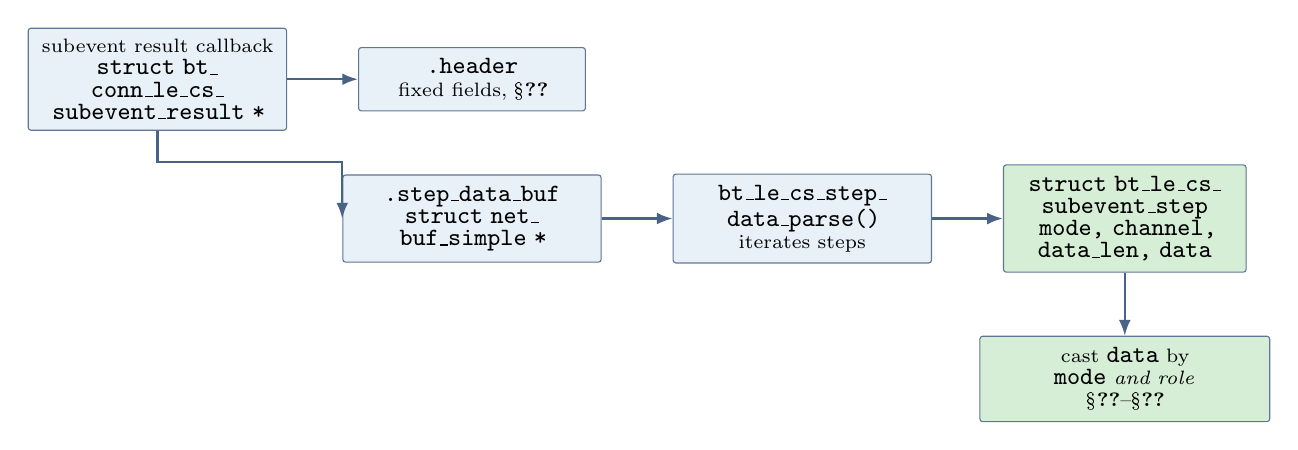
\begin{tikzpicture}[node distance=5mm and 9mm]
\node[blk,text width=30mm] (cb) {subevent result callback\\ \code{struct bt\_\allowbreak{}conn\_\allowbreak{}le\_\allowbreak{}cs\_\allowbreak{}subevent\_\allowbreak{}result *}};
\node[blk,right=of cb,text width=26mm] (hdr) {\code{.header}\\ fixed fields, \S\ref{sec:header}};
\node[blk,below=8mm of hdr,text width=30mm] (buf) {\code{.step\_\allowbreak{}data\_\allowbreak{}buf}\\ \code{struct net\_\allowbreak{}buf\_\allowbreak{}simple *}};
\node[blk,right=of buf,text width=30mm] (parse) {\code{bt\_\allowbreak{}le\_\allowbreak{}cs\_\allowbreak{}step\_\allowbreak{}data\_\allowbreak{}parse()}\\ iterates steps};
\node[gblk,right=of parse,text width=28mm] (step) {\code{struct bt\_\allowbreak{}le\_\allowbreak{}cs\_\allowbreak{}subevent\_\allowbreak{}step}\\ \code{mode, channel, data\_\allowbreak{}len, data}};
\node[gblk,below=8mm of step,text width=34mm] (cast) {cast \code{data} by \code{mode} \emph{and role}\\ \S\ref{sec:mode0}--\S\ref{sec:mode3}};
\draw[ar] (cb)--(hdr);
\draw[ar] (cb.south) -- ++(0,-4mm) -| (buf.west);
\draw[ar] (buf)--(parse); \draw[ar] (parse)--(step); \draw[ar] (step)--(cast);
\end{tikzpicture}
\caption{From callback to a single interpreted step. The header is typed; the step payload is not ---
its layout is determined by the step mode \emph{and} by the local device's role, neither of which is
carried inside the payload itself.}
\label{fig:path}
\end{figure}

\subsection{The subevent result}

\begin{lstlisting}
struct bt_conn_le_cs_subevent_result {
        struct {
                uint8_t  config_id;
                uint16_t start_acl_conn_event;
                uint16_t procedure_counter;
                uint16_t frequency_compensation;
                int8_t   reference_power_level;
                enum bt_conn_le_cs_procedure_done_status  procedure_done_status;
                enum bt_conn_le_cs_subevent_done_status   subevent_done_status;
                enum bt_conn_le_cs_procedure_abort_reason procedure_abort_reason;
                enum bt_conn_le_cs_subevent_abort_reason  subevent_abort_reason;
                uint8_t  num_antenna_paths;
                uint8_t  num_steps_reported;
                uint8_t  abort_step;
        } header;
        /* NULL if num_steps_reported is 0 */
        struct net_buf_simple *step_data_buf;
};
\end{lstlisting}

\subsection{The step iterator}

\begin{lstlisting}
void bt_le_cs_step_data_parse(struct net_buf_simple *step_data_buf,
                              bool (*func)(struct bt_le_cs_subevent_step *step,
                                           void *user_data),
                              void *user_data);

struct bt_le_cs_subevent_step {
        uint8_t        mode;
        uint8_t        channel;
        uint8_t        data_len;
        const uint8_t *data;
};
\end{lstlisting}

The callback returns \code{true} to continue iterating and \code{false} to stop. Note what
\code{struct bt\_\allowbreak{}le\_\allowbreak{}cs\_\allowbreak{}subevent\_\allowbreak{}step} contains and, more importantly, what it does not: there is
no step index, no role, and no indication of which layout variant \code{data} holds. The step index
must be maintained by the caller as an iteration counter --- and it matters, because
\code{header.abort\_\allowbreak{}step} is expressed in it.

\subsection{The phase correction term helper}

\begin{lstlisting}
struct bt_le_cs_iq_sample {
        int16_t i;
        int16_t q;
};

/* Sign-extends the 12-bit I and Q halves of a 3-octet phase correction term. */
struct bt_le_cs_iq_sample bt_le_cs_parse_pct(const uint8_t pct[3]);
\end{lstlisting}

\begin{callout}
\textbf{Use the helper; do not unpack the term by hand.} The phase correction term packs two
\emph{signed} 12-bit values into three octets \core{Vol.\ 4, Part E}. A hand-rolled unpack that masks
without sign-extending yields values in $[0,4095]$ instead of $[-2048,2047]$, which silently folds
the negative half-plane onto the positive one. Every phase in the lower half of the complex plane
then comes out wrong, and the resulting range is wrong without being obviously so.
\end{callout}

% ============================================================
\section{The subevent header}
\label{sec:header}
% ============================================================

\begin{table}[htb]
\caption{Subevent header fields. Ranges, units and unavailable encodings are from
\core{Vol.\ 4, Part E, LE CS Subevent Result}.}
\label{tab:header}
\centering\scriptsize
\begin{tabular}{@{}L{34mm}L{50mm}L{54mm}@{}}
\toprule
Zephyr field & Specification meaning & Use, and companion-report symbol \\
\midrule
\code{config\_\allowbreak{}id} & CS configuration identifier, 0--3. Zero and meaningless for CS Test results & Store: identifies which configuration the geometry belongs to \\
\code{start\_\allowbreak{}acl\_\allowbreak{}conn\_\allowbreak{}event} & Starting ACL connection event counter & Store: ties the subevent to the connection timeline \\
\code{procedure\_\allowbreak{}counter} & CS procedure count since the CS Security Start procedure & \textbf{Primary grouping key.} All steps of one procedure share it \\
\code{frequency\_\allowbreak{}compensation} & \code{Frequency\_\allowbreak{}Compensation}: 15-bit signed, units $0.01$\,ppm, range $\pm100$\,ppm. \code{0xC000} = unavailable \emph{or} role is not initiator & The subevent frequency reference: $\FFO^{*}_{RX}$ of the Mode-0 report. Divide by 100 for ppm; this is $\varepsilon\times10^{6}$ \\
\code{reference\_\allowbreak{}power\_\allowbreak{}level} & \code{Reference\_\allowbreak{}Power\_\allowbreak{}Level}: dBm, range $-127$ to $20$; \code{0x7F} not applicable & $\RPL$ of the Mode-2 report. Needed to convert $\PCT$ magnitude to dBm, Eq.~\eqref{eq:rpl} \\
\code{procedure\_\allowbreak{}done\_\allowbreak{}status} & Complete / partial / aborted & Gate: only combine procedures whose status you trust \\
\code{subevent\_\allowbreak{}done\_\allowbreak{}status} & Complete / aborted & Gate \\
\code{procedure\_\allowbreak{}abort\_\allowbreak{}reason} & No abort, requested, too few channels, channel-map instant passed, unspecified & Diagnostic; ``too few channels'' directly explains a degraded aperture \\
\code{subevent\_\allowbreak{}abort\_\allowbreak{}reason} & No abort, requested, no \code{CS\_\allowbreak{}SYNC} received, scheduling conflict, unspecified & Diagnostic \\
\code{num\_\allowbreak{}antenna\_\allowbreak{}paths} & \code{Num\_\allowbreak{}Antenna\_\allowbreak{}Paths}: 0 means no phase measurement in the step; otherwise 1--4 & $\Nap$. \textbf{Determines the tone array length}, which is $\Nap+1$ \\
\code{num\_\allowbreak{}steps\_\allowbreak{}reported} & Number of CS steps in the subevent & Loop bound; cross-check against the iterator count \\
\code{abort\_\allowbreak{}step} & Step number at which the subevent aborted; 255 when complete & Steps $0\ldots\text{\code{abort\_\allowbreak{}step}}-1$ are valid; the rest are not \\
\bottomrule
\end{tabular}
\end{table}

\begin{caution}
\textbf{Two header fields are sentinels, not numbers.} \code{frequency\_\allowbreak{}compensation} is
\code{0xC000} when unavailable \emph{or} when the local device is the reflector, and
\code{reference\_\allowbreak{}power\_\allowbreak{}level} is \code{0x7F} when not applicable. Both are in range for their
declared types and neither is flagged separately. Testing for them before use is not defensive
programming; it is required, because \code{0xC000} interpreted as a signed $0.01$\,ppm value is
$-163.84$\,ppm, which exceeds the specification's own $\pm50$\,ppm bound on a Mode-0 step and would
be applied as a frequency correction fifteen hundred times larger than a realistic one.
\end{caution}

\subsection{The two frequency quantities are not the same}

The header's \code{frequency\_\allowbreak{}compensation} and the mode-0 step's \code{measured\_\allowbreak{}freq\_\allowbreak{}offset} share
units and encoding and are easily conflated. They are different quantities in the Mode-0 report's
terms.

\begin{table}[h]
\caption{The two fractional frequency quantities.}
\label{tab:twofreq}
\centering\small
\begin{tabular}{@{}L{34mm}L{40mm}L{30mm}L{34mm}@{}}
\toprule
 & Where & Scope & Companion symbol \\
\midrule
\code{measured\_\allowbreak{}freq\_\allowbreak{}offset} & Mode-0 step, initiator only & One mode-0 step, one channel & $\FFO_{RX}[k]$ \\
\code{frequency\_\allowbreak{}compensation} & Subevent header & The subevent; what the controller actually applied & $\FFO^{*}_{RX}$ \\
\bottomrule
\end{tabular}
\end{table}

Store both. The per-step values let you assess the Mode-0 report's combining rule and detect the
channel-correlated spread that indicates a stale actuation-error table; the subevent value is what
the controller used, and is therefore the one that already influenced the mode-1, mode-2 and mode-3
steps you are about to process.
% ============================================================
\section{Mode-0 step data}
\label{sec:mode0}
% ============================================================

Mode-0 is the only mode whose layout differs by role in the number of fields, because only the
initiator measures a frequency offset \core{Vol.\ 6, Part H, Sec.\ 4.3.1}.

\begin{lstlisting}
struct bt_hci_le_cs_step_data_mode_0_initiator {
        uint8_t  packet_quality_bit_errors : 4;
        uint8_t  packet_quality_aa_check   : 4;
        uint8_t  packet_rssi;
        uint8_t  packet_antenna;
        uint16_t measured_freq_offset;
} __packed;

struct bt_hci_le_cs_step_data_mode_0_reflector {
        uint8_t packet_quality_bit_errors : 4;
        uint8_t packet_quality_aa_check   : 4;
        uint8_t packet_rssi;
        uint8_t packet_antenna;
} __packed;
\end{lstlisting}

\begin{table}[h]
\caption{Mode-0 step fields.}
\label{tab:mode0}
\centering\scriptsize
\begin{tabular}{@{}L{32mm}L{56mm}L{50mm}@{}}
\toprule
Zephyr field & Specification meaning & Use, and companion symbol \\
\midrule
\code{packet\_\allowbreak{}quality\_\allowbreak{}aa\_\allowbreak{}check} & \code{Packet\_\allowbreak{}Quality} bits 0--3: \code{0x0} access address matched exactly, \code{0x1} one or more bit errors, \code{0x2} access address not found & Primary gate. Anything but \code{0x0} means the timing reference for the subevent is suspect \\
\code{packet\_\allowbreak{}quality\_\allowbreak{}bit\_\allowbreak{}errors} & \code{Packet\_\allowbreak{}Quality} bits 4--7: payload bit-error count when the RTT type carries a random or sounding sequence; 0 may mean zero errors \emph{or} no report; 15 means 15 or more & Mode-0 packets carry no sequence, so this is not meaningful here \\
\code{packet\_\allowbreak{}rssi} & \code{Packet\_\allowbreak{}RSSI}: dBm, $-127$ to $+20$; \code{0x7F} unavailable & Signal-to-noise proxy $\gamma$ for the Mode-0 report's Cram\'er--Rao bound \\
\code{packet\_\allowbreak{}antenna} & \code{Packet\_\allowbreak{}Antenna}: antenna identifier \code{0x01}--\code{0x04} used for the \code{CS\_\allowbreak{}SYNC} & Calibration selection \\
\code{measured\_\allowbreak{}freq\_\allowbreak{}offset} & \code{Measured\_\allowbreak{}Freq\_\allowbreak{}Offset}: 15-bit signed, units $0.01$\,ppm, range $\pm100$\,ppm; \code{0xC000} unavailable. Defined as $\FFO[k]$ of \core{Vol.\ 6, Part A, Sec.\ 3.5.1} & $\FFO_{RX}[k]$. \textbf{Initiator only} \\
\bottomrule
\end{tabular}
\end{table}

\begin{callout}
\textbf{What the specification says this field \emph{is}.} Core 6.3 states that
``the \code{Measured\_\allowbreak{}Freq\_\allowbreak{}Offset} parameter indicates the value of the FFO measured by the
initiator device during the mode-0 CS step (see FFO[k] in [Vol 6] Part A, Section 3.5.1)''. That is
exactly the quantity the Mode-0 report derives, so the mapping is an identity rather than an
interpretation: the controller has already performed the reconstruction from baseband beat to
received frequency, applied its own local actuation error, and removed the peer's actuation error
from the table. What reaches you is $\varepsilon$ in hundredths of a part per million.
\end{callout}

Converting to the report's dimensionless $\varepsilon$:
\begin{equation}
\varepsilon \;=\; \frac{\texttt{\footnotesize measured\_freq\_offset}}{100}\times10^{-6},
\label{eq:ffoconv}
\end{equation}
after sign-extending the 15-bit value and rejecting \code{0xC000}.

% ============================================================
\section{Mode-1 step data}
\label{sec:mode1}
% ============================================================

\begin{lstlisting}
struct bt_hci_le_cs_step_data_mode_1 {
        uint8_t packet_quality_bit_errors : 4;
        uint8_t packet_quality_aa_check   : 4;
        uint8_t packet_nadm;
        uint8_t packet_rssi;
        union {
                int16_t toa_tod_initiator;   /* valid when local role is initiator */
                int16_t tod_toa_reflector;   /* valid when local role is reflector */
        };
        uint8_t packet_antenna;
} __packed;
\end{lstlisting}

\begin{table}[htb]
\caption{Mode-1 step fields. Fields shared with mode-0 are not repeated.}
\label{tab:mode1}
\centering\scriptsize
\begin{tabular}{@{}L{32mm}L{56mm}L{50mm}@{}}
\toprule
Zephyr field & Specification meaning & Use, and companion symbol \\
\midrule
\code{packet\_\allowbreak{}quality\_\allowbreak{}bit\_\allowbreak{}errors} & Payload bit errors, 0--15, meaningful when the RTT type carries a random or sounding sequence & Quality weight for the timing estimate \\
\code{packet\_\allowbreak{}nadm} & \code{Packet\_\allowbreak{}NADM}: \code{0x00} attack extremely unlikely through \code{0x06} extremely likely; \code{0xFF} unknown, and the default for RTT types with no random or sounding sequence & $\NADM$ of the Mode-1 report. Integrity gate \\
\code{toa\_\allowbreak{}tod\_\allowbreak{}initiator} & \code{ToA\_\allowbreak{}ToD\_\allowbreak{}Initiator}: signed 16-bit, units $0.5$\,ns, \textbf{known nominal offsets omitted}; \code{0x8000} unavailable & Yields $A_I$ of the Mode-1 report once the nominal offsets are restored, Eq.~\eqref{eq:restore} \\
\code{tod\_\allowbreak{}toa\_\allowbreak{}reflector} & \code{ToD\_\allowbreak{}ToA\_\allowbreak{}Reflector}: same encoding, reflector side & Yields $B_R$ \\
\bottomrule
\end{tabular}
\end{table}

\subsection{The omitted nominal offsets}

This is the single most consequential detail in the whole mapping, and the specification states it
explicitly: the reported value is the time difference ``where the known nominal offsets are omitted.
The known offsets (i.e., the interlude time between packets and the length of the packet itself) are
described in [Vol 6] Part H, Section 4.3.2 and [Vol 6] Part H, Section 4.3.4 for Mode-1 and Mode-3''
\core{Vol.\ 4, Part E}.

The controller therefore reports a \emph{residual} about the configured nominal step timing, not the
absolute interval the Mode-1 report's $A_I$ and $B_R$ denote. To recover them:
\begin{align}
A_I &= \underbrace{\bigl(\Tsy + \Trd + T_{IP1}\bigr)}_{\text{nominal, from the configuration}}
       \;+\; 0.5\,\text{ns}\times\text{\code{toa\_\allowbreak{}tod\_\allowbreak{}initiator}} , \label{eq:restore}\\
B_R &= \bigl(\Tsy + \Trd + T_{IP1}\bigr)
       \;+\; 0.5\,\text{ns}\times\text{\code{tod\_\allowbreak{}toa\_\allowbreak{}reflector}} ,
\end{align}
for a Mode-1 step, with the corresponding Mode-3 nominal from that report's step structure. The
round-trip time of the Mode-1 report then follows as $\RTT = A_I - \tilde B_R - \hat D_{loop}$.

\begin{callout}
\textbf{Why this closes an open question.} The Mode-1 report's host-interface appendix observed that
a signed 16-bit field at $0.5$\,ns resolution spans only about $\pm16.4\us$, far narrower than the
largest permitted interlude period, and concluded that the reported quantity ``is therefore a
differential referenced to the configured nominal step timing rather than an absolute interval'', to
be confirmed against the specification. It is confirmed. The practical consequence is that
\textbf{the nominal step timing is part of the measurement} --- you cannot reconstruct a range from
the step reports alone, and a stored procedure whose timing configuration was not stored with it is
not reducible later.
\end{callout}

\subsection{The variant the documented structure does not show}
\label{sec:m1variant}

Core 6.3 defines the mode-1 role-specific information to carry two additional fields when the
conditions are right. For an initiator, ``when the mode type is 1, the role is initiator, sounding
phase-based ranging is supported, and the RTT type contains a sounding sequence'', the parameters are
\code{Packet\_\allowbreak{}Quality}, \code{Packet\_\allowbreak{}NADM}, \code{Packet\_\allowbreak{}RSSI}, \code{ToA\_\allowbreak{}ToD\_\allowbreak{}Initiator},
\code{Packet\_\allowbreak{}Antenna}, \code{Packet\_\allowbreak{}PCT1} and \code{Packet\_\allowbreak{}PCT2} \core{Vol.\ 4, Part E}.

\begin{table}[h]
\caption{The mode-1 sounding-sequence phase fields.}
\label{tab:pct12}
\centering\small
\begin{tabular}{@{}L{28mm}L{58mm}L{52mm}@{}}
\toprule
Field & Encoding & Meaning \\
\midrule
\code{Packet\_\allowbreak{}PCT1} & 4 octets: bits 0--11 $I$ (\code{sint12}), bits 12--23 $Q$ (\code{sint12}), bits 24--31 reserved; \code{0xFFFFFFFF} unavailable & Phase measured on the sounding sequence of the \code{CS\_\allowbreak{}SYNC} \\
\code{Packet\_\allowbreak{}PCT2} & Identical encoding & Second such term \\
\bottomrule
\end{tabular}
\end{table}

This is phase-based ranging extracted from the RTT packet's sounding sequence rather than from tones
--- the capability advertised as ``CS phase-based ranging from RTT sounding sequence'' and referred to
in \core{Vol.\ 6, Part A, Sec.\ 6.3} where the local actuation-error phase correction is applied over
\code{T\_\allowbreak{}SY\_\allowbreak{}CENTER\_\allowbreak{}DELTA}. The documented Zephyr \code{bt\_\allowbreak{}hci\_\allowbreak{}le\_\allowbreak{}cs\_\allowbreak{}step\_\allowbreak{}data\_\allowbreak{}mode\_\allowbreak{}1}
structure does not include these fields.

\begin{caution}
\textbf{Do not size a mode-1 step from \code{sizeof()}.} Because the presence of the two phase
correction terms depends on role, on capability and on the configured RTT type, a mode-1 step record
has more than one length. \code{step->data\_\allowbreak{}len} is the authority. An application that casts blindly
and advances by \code{sizeof(struct bt\_\allowbreak{}hci\_\allowbreak{}le\_\allowbreak{}cs\_\allowbreak{}step\_\allowbreak{}data\_\allowbreak{}mode\_\allowbreak{}1)} will misparse every
subsequent step in a configuration that carries the extra fields --- and the Zephyr iterator does not
protect you, because it advances by the length the controller reported, not by your struct size.
Compare \code{data\_\allowbreak{}len} against the expected length for your configuration and reject a mismatch
rather than interpreting it.
\end{caution}
% ============================================================
\section{Mode-2 step data}
\label{sec:mode2}
% ============================================================

\begin{lstlisting}
struct bt_hci_le_cs_step_data_tone_info {
        uint8_t phase_correction_term[3];  /* 12-bit I, 12-bit Q, packed */
        uint8_t extension_indicator : 4;
        uint8_t quality_indicator   : 4;
} __packed;

struct bt_hci_le_cs_step_data_mode_2 {
        uint8_t antenna_permutation_index;
        struct bt_hci_le_cs_step_data_tone_info tone_info[];  /* N_AP + 1 entries */
} __packed;
\end{lstlisting}

\begin{table}[htb]
\caption{Mode-2 step fields.}
\label{tab:mode2}
\centering\scriptsize
\begin{tabular}{@{}L{32mm}L{56mm}L{50mm}@{}}
\toprule
Zephyr field & Specification meaning & Use, and companion symbol \\
\midrule
\code{antenna\_\allowbreak{}permutation\_\allowbreak{}index} & \code{Antenna\_\allowbreak{}Path\_\allowbreak{}Permutation\_\allowbreak{}Index}: which permutation of antenna paths this step used & Maps tone slot to physical antenna path. The Mode-2 report's ``silent and fatal'' failure if mis-applied \\
\code{tone\_\allowbreak{}info[k]} & \code{Tone\_\allowbreak{}PCT[k]}, size $(\Nap+1)\times3$ octets & The array length is $\Nap+1$, from the \emph{header's} \code{num\_\allowbreak{}antenna\_\allowbreak{}paths} \\
\code{.phase\_\allowbreak{}correction\_\allowbreak{}term} & Bits 0--11 $I$ (\code{sint12}), 12--23 $Q$ (\code{sint12}); with \IPT{} enabled on the reflector, $Q$ is set to $0$ & $\PCT_{INIT}(f_k)$ or $\PCT_{REFL}(f_k)$ of the Mode-2 report \\
\code{.quality\_\allowbreak{}indicator} & \code{Tone\_\allowbreak{}Quality\_\allowbreak{}Indicator[k]} bits 0--3: tone quality per \core{Vol.\ 6, Part H, Sec.\ 4.6} & $\TQI$. Gating and weighting input \\
\code{.extension\_\allowbreak{}indicator} & \code{Tone\_\allowbreak{}Quality\_\allowbreak{}Indicator[k]} bits 4--7: whether the slot is a tone extension slot and whether it was expected to carry a transmission & Identifies the extension slot, which must be excluded from any slope fit \\
\bottomrule
\end{tabular}
\end{table}

\begin{caution}
\textbf{The tone array is $\Nap+1$ long, and the last entry is not a measurement.} The extra slot is
the tone extension slot. The Mode-2 report treats it as the step's own noise and interference
reference --- valuable, and the only same-step, same-gain noise estimate available --- but it is not
an antenna path and it must not enter a phase-slope fit or a transform. Read
\code{extension\_\allowbreak{}indicator} rather than assuming the last index, because the specification describes
it as indicating both \emph{whether} a slot is an extension slot and whether a transmission was
expected in it, and the reflector's extension slot may legitimately carry no transmission at all.
\end{caution}

\subsection{Forming the two-way phase}

The Mode-2 report's central operation, restated in API terms. For channel $k$ and antenna path $p$,
with \code{ii} and \code{qq} the sign-extended halves from \code{bt\_\allowbreak{}le\_\allowbreak{}cs\_\allowbreak{}parse\_\allowbreak{}pct}:
\begin{equation}
H_2(f_k,p) \;=\; \PCT_{INIT}(f_k,p)\;\PCT_{REFL}(f_k,p),
\qquad
\Theta(f_k,p) \;=\; \arg H_2(f_k,p) .
\label{eq:twoway}
\end{equation}
Multiply the two complex numbers. Do not convert each to an angle and add: an isolated
\code{atan2} result is wrapped, and the sum of two wrapped angles is not the wrapped sum.

\begin{callout}
\textbf{Both devices' terms are needed, and only one of them arrives locally.} A subevent result
delivers the \emph{local} device's phase correction terms. Equation~\eqref{eq:twoway} needs the
peer's as well, which must reach the ranging entity by some other path --- unless Inline Phase
Transfer is enabled, in which case the reflector has pre-rotated its carrier, its reported $Q$ is
zero by requirement, and the initiator's own term already carries $2\theta_{CH}$. That is the whole
subject of the companion \IPT{} report, and it changes what you must store: with \IPT{} the
reflector's term contributes amplitude only.
\end{callout}

Converting a term's magnitude to power, per \core{Vol.\ 6, Part H, Sec.\ 4.6}:
\begin{equation}
P_{\mathrm{dBm}} \;=\; 20\log_{10}\!\left(\frac{\sqrt{I^2+Q^2}}{2048}\right) \;+\; \RPL_{\mathrm{dBm}} ,
\label{eq:rpl}
\end{equation}
with $\RPL$ the header's \code{reference\_\allowbreak{}power\_\allowbreak{}level}, one value for the whole subevent.

% ============================================================
\section{Mode-3 step data}
\label{sec:mode3}
% ============================================================

\begin{lstlisting}
struct bt_hci_le_cs_step_data_mode_3 {
        uint8_t packet_quality_bit_errors : 4;
        uint8_t packet_quality_aa_check   : 4;
        uint8_t packet_nadm;
        uint8_t packet_rssi;
        union {
                int16_t toa_tod_initiator;
                int16_t tod_toa_reflector;
        };
        uint8_t packet_antenna;
        uint8_t antenna_permutation_index;
        struct bt_hci_le_cs_step_data_tone_info tone_info[];  /* N_AP + 1 entries */
} __packed;
\end{lstlisting}

Mode-3 is the concatenation of the mode-1 and mode-2 field sets, and every field carries the meaning
already given in Tables~\ref{tab:mode1} and~\ref{tab:mode2}. The same
\code{Packet\_\allowbreak{}PCT1}/\code{Packet\_\allowbreak{}PCT2} variant exists here as in mode-1, under the same conditions
\core{Vol.\ 4, Part E}, and the same warning about \code{data\_\allowbreak{}len} applies with more force because a
mode-3 record has more optional content.

\begin{callout}
\textbf{What mode-3 uniquely enables, in storage terms.} Because the timing and phase fields arrive
in one record, they are known to share a channel, an antenna path permutation, a gain state and an
instant. That is the premise of the companion Mode-3 report's per-channel seeded unwrap and of its
cross-observable consistency residual $\delta_k = \hat d_{\RTT,k} - \hat d_{\Theta,k}$. Preserve the
pairing: store the timing and tone fields of a mode-3 step in one row, never in two tables joined
later on channel, because a join on channel across a procedure silently reintroduces exactly the
mismatch mode-3 exists to remove.
\end{callout}

% ============================================================
\section{Master mapping}
\label{sec:master}
% ============================================================

\begin{table}[htb]
\caption{Every result field, in all three vocabularies. ``Report'' cites the companion document in
which the quantity is developed.}
\label{tab:master}
\centering\scriptsize
\begin{tabular}{@{}L{31mm}L{31mm}L{24mm}L{18mm}L{28mm}@{}}
\toprule
Zephyr & Core 6.3 HCI & Symbol & Report & Unavailable \\
\midrule
\code{procedure\_\allowbreak{}counter} & \code{Procedure\_\allowbreak{}Counter} & --- & --- & --- \\
\code{frequency\_\allowbreak{}compensation} & \code{Frequency\_\allowbreak{}Compensation} & $\FFO^{*}_{RX}$ & Mode-0 & \code{0xC000} \\
\code{reference\_\allowbreak{}power\_\allowbreak{}level} & \code{Reference\_\allowbreak{}Power\_\allowbreak{}Level} & $\RPL$ & Mode-2 & \code{0x7F} \\
\code{num\_\allowbreak{}antenna\_\allowbreak{}paths} & \code{Num\_\allowbreak{}Antenna\_\allowbreak{}Paths} & $\Nap$ & Mode-2/3 & \code{0x00} = none \\
\code{num\_\allowbreak{}steps\_\allowbreak{}reported} & \code{Num\_\allowbreak{}Steps\_\allowbreak{}Reported} & $M$, $K$ & all & --- \\
\code{abort\_\allowbreak{}step} & --- & --- & --- & \code{255} = none \\
\code{step->mode} & \code{Step\_\allowbreak{}Mode} & --- & all & --- \\
\code{step->channel} & \code{Step\_\allowbreak{}Channel} & $f_k$ index & Mode-2/3 & --- \\
\code{packet\_\allowbreak{}quality\_\allowbreak{}aa\_\allowbreak{}check} & \code{Packet\_\allowbreak{}Quality} bits 0--3 & --- & all & --- \\
\code{packet\_\allowbreak{}quality\_\allowbreak{}bit\_\allowbreak{}errors} & \code{Packet\_\allowbreak{}Quality} bits 4--7 & --- & Mode-1/3 & 0 ambiguous \\
\code{packet\_\allowbreak{}nadm} & \code{Packet\_\allowbreak{}NADM} & $\NADM$ & Mode-1/3 & \code{0xFF} \\
\code{packet\_\allowbreak{}rssi} & \code{Packet\_\allowbreak{}RSSI} & $\gamma$ proxy & all & \code{0x7F} \\
\code{packet\_\allowbreak{}antenna} & \code{Packet\_\allowbreak{}Antenna} & --- & all & --- \\
\code{measured\_\allowbreak{}freq\_\allowbreak{}offset} & \code{Measured\_\allowbreak{}Freq\_\allowbreak{}Offset} & $\FFO_{RX}[k]$ & Mode-0 & \code{0xC000} \\
\code{toa\_\allowbreak{}tod\_\allowbreak{}initiator} & \code{ToA\_\allowbreak{}ToD\_\allowbreak{}Initiator} & $A_I$ (residual) & Mode-1/3 & \code{0x8000} \\
\code{tod\_\allowbreak{}toa\_\allowbreak{}reflector} & \code{ToD\_\allowbreak{}ToA\_\allowbreak{}Reflector} & $B_R$ (residual) & Mode-1/3 & \code{0x8000} \\
--- (variant) & \code{Packet\_\allowbreak{}PCT1/2} & --- & \S\ref{sec:m1variant} & \code{0xFFFFFFFF} \\
\code{antenna\_\allowbreak{}permutation\_\allowbreak{}index} & \code{Antenna\_\allowbreak{}Path\_\allowbreak{}Permutation\_\allowbreak{}Index} & --- & Mode-2/3 & --- \\
\code{phase\_\allowbreak{}correction\_\allowbreak{}term} & \code{Tone\_\allowbreak{}PCT[k]} & $\PCT(f_k)$ & Mode-2/3, \IPT & --- \\
\code{quality\_\allowbreak{}indicator} & \code{Tone\_\allowbreak{}Quality\_\allowbreak{}Indicator} bits 0--3 & $\TQI$ & Mode-2/3 & unavailable code \\
\code{extension\_\allowbreak{}indicator} & \code{Tone\_\allowbreak{}Quality\_\allowbreak{}Indicator} bits 4--7 & --- & Mode-2/3 & --- \\
\bottomrule
\end{tabular}
\end{table}
% ============================================================
\section{What to store}
\label{sec:store}
% ============================================================

One principle governs the schema: \textbf{persist what the controller reported, derive nothing
irreversibly.} Every correction in the companion reports is one an implementation revises --- the
loop-delay calibration surface is refined, the actuation-error table is refreshed, the unwrap is
re-seeded, the first-path threshold is re-characterised. A stored range is a dead end; a stored step
report can be re-reduced with next year's calibration.

\subsection{Configuration context, stored once per procedure}

This is the layer most easily forgotten, and Section~\ref{sec:mode1} shows why it is not optional:
without the nominal step timing the reported timing residuals cannot be turned into intervals at all.
Section~\ref{sec:config} documents where each of these values comes from; the short version is that
the ones that matter most are reported once and never again.

\begin{table}[h]
\caption{Per-procedure context. None of this arrives in the subevent result; all of it is needed to
reduce one. Section~\ref{sec:config} documents each source, and Table~\ref{tab:latch} says which of
them cannot be recovered after the fact.}
\label{tab:ctx}
\centering\scriptsize
\begin{tabular}{@{}L{46mm}L{44mm}L{48mm}@{}}
\toprule
Item & Source & Why it is needed \\
\midrule
Local role (initiator / reflector) & \code{bt\_\allowbreak{}conn\_\allowbreak{}le\_\allowbreak{}cs\_\allowbreak{}config.role} & Decides which union member is valid and which mode-0 layout applies \\
\code{config\_\allowbreak{}id}, \code{procedure\_\allowbreak{}counter} & Header, plus the security session (\S\ref{sec:setuporder}) & Grouping keys \\
Main and sub mode, RTT type & \code{bt\_\allowbreak{}conn\_\allowbreak{}le\_\allowbreak{}cs\_\allowbreak{}config} & Decides step layout and whether the \code{Packet\_\allowbreak{}PCT} variant is present \\
$T_{IP1}$, $T_{IP2}$, $T_{FCS}$, $\Tpm$ & \code{bt\_\allowbreak{}conn\_\allowbreak{}le\_\allowbreak{}cs\_\allowbreak{}config}, \emph{negotiated} (\S\ref{sec:cfgtimes}) & Restoring the omitted nominal offsets, Eq.~\eqref{eq:restore} \\
$\Tsw$ & Capability exchange, \emph{not} the config event (\S\ref{sec:cfgtimes}) & Tone slot duration $(\Tsw+\Tpm)(\Nap+1)$; antenna switching \\
$\Trd$ & Fixed $5$\us & Nominal offset term \\
CS PHY & \code{bt\_\allowbreak{}conn\_\allowbreak{}le\_\allowbreak{}cs\_\allowbreak{}config.cs\_\allowbreak{}sync\_\allowbreak{}phy} & $\Tsy$, and $\beta_{rms}$ for the Mode-1 bound \\
Antenna configuration index, $\Nap$ & \code{procedure\_\allowbreak{}enable\_\allowbreak{}complete} and header & Tone array length; per-path calibration \\
Channel map actually used & \code{bt\_\allowbreak{}conn\_\allowbreak{}le\_\allowbreak{}cs\_\allowbreak{}config.channel\_\allowbreak{}map}, narrowed by classification & The aperture. The Mode-2 report shows the largest gap sets the unwrap limit \\
Scheduling cadence & \code{procedure\_\allowbreak{}enable\_\allowbreak{}complete} (\S\ref{sec:procenable}) & The measurement time base; granted values differ from requested \\
\IPT{} enabled & \code{cs\_\allowbreak{}enhancements\_\allowbreak{}1} bit 0 & Whether the reflector's $Q$ is meaningful \\
Calibration versions: $D_{loop}$, $\Phi_{loop}(f)$, $\FAE$ table & Your own state; $\FAE$ from \S\ref{sec:fae} & Reproducibility of any later re-reduction \\
\bottomrule
\end{tabular}
\end{table}

\subsection{Per subevent}

Every header field of Table~\ref{tab:header}, without exception, plus a local receive timestamp. The
status and abort fields are small and are the only record of why a procedure was thin.

\subsection{Per step}

Store the step index (the iterator count), \code{mode}, \code{channel}, \code{data\_\allowbreak{}len}, and the
decoded fields for that mode. Three storage rules earn their place:

\begin{enumerate}[leftmargin=1.6em,itemsep=2pt]
  \item \textbf{Store raw integers, not converted physical values.} Keep
    \code{measured\_\allowbreak{}freq\_\allowbreak{}offset} as the signed count of $0.01$\,ppm and
    \code{toa\_\allowbreak{}tod\_\allowbreak{}initiator} as the signed count of $0.5$\,ns. Conversions are cheap to redo and
    impossible to undo, and a stored float has already lost the sentinel.
  \item \textbf{Store sentinels as null, and store the fact separately.} Do not coerce \code{0x8000}
    or \code{0xC000} into a number. A boolean ``available'' column beside each such field makes every
    later query safe by construction.
  \item \textbf{Keep the tone array ordered and complete}, including the extension slot, with its
    \code{extension\_\allowbreak{}indicator}. The Mode-2 report wants the extension slot as a noise reference;
    discarding it at ingest throws away the only same-step noise estimate.
  \end{enumerate}

\begin{table}[h]
\caption{Minimum per-step record by mode. \checkmark\ = store; --- = not present.}
\label{tab:store}
\centering\scriptsize
\begin{tabular}{@{}L{44mm}cccc@{}}
\toprule
Field & Mode-0 & Mode-1 & Mode-2 & Mode-3 \\
\midrule
step index, mode, channel, \code{data\_\allowbreak{}len} & \checkmark & \checkmark & \checkmark & \checkmark \\
\code{packet\_\allowbreak{}quality\_\allowbreak{}aa\_\allowbreak{}check} & \checkmark & \checkmark & --- & \checkmark \\
\code{packet\_\allowbreak{}quality\_\allowbreak{}bit\_\allowbreak{}errors} & \checkmark & \checkmark & --- & \checkmark \\
\code{packet\_\allowbreak{}rssi} & \checkmark & \checkmark & --- & \checkmark \\
\code{packet\_\allowbreak{}antenna} & \checkmark & \checkmark & --- & \checkmark \\
\code{measured\_\allowbreak{}freq\_\allowbreak{}offset} (initiator) & \checkmark & --- & --- & --- \\
\code{packet\_\allowbreak{}nadm} & --- & \checkmark & --- & \checkmark \\
timing residual (\code{toa\_\allowbreak{}tod}/\code{tod\_\allowbreak{}toa}) & --- & \checkmark & --- & \checkmark \\
\code{Packet\_\allowbreak{}PCT1/2} if the variant is configured & --- & \checkmark & --- & \checkmark \\
\code{antenna\_\allowbreak{}permutation\_\allowbreak{}index} & --- & --- & \checkmark & \checkmark \\
per tone: $I$, $Q$, \code{quality\_\allowbreak{}indicator}, \code{extension\_\allowbreak{}indicator} & --- & --- & \checkmark & \checkmark \\
\bottomrule
\end{tabular}
\end{table}

\subsection{Derived values, stored alongside and never in place of the raw}

Range estimates, $\varepsilon$, $\Theta(f_k)$, unwrap decisions and their seeds, gate outcomes and
the calibration version used. The Mode-3 report's consistency residual $\delta_k$ belongs here too.
Storing the \emph{decisions} as well as the results is what makes a later disagreement diagnosable.

% ============================================================
\section{How to use each report}
\label{sec:use}
% ============================================================

\subsection{Mode-0: establish the scale, then gate on it}

Take \code{measured\_\allowbreak{}freq\_\allowbreak{}offset} from each mode-0 step whose \code{packet\_\allowbreak{}quality\_\allowbreak{}aa\_\allowbreak{}check} is
\code{0x0}, convert with Eq.~\eqref{eq:ffoconv}, and combine across the one to three mode-0 steps of
the subevent. Compare the result against the header's \code{frequency\_\allowbreak{}compensation}, which is what
the controller actually applied. The Mode-0 report's checks apply directly: a spread across steps
that correlates with channel indicates a stale or mis-indexed actuation-error table, and the
specification's own bound is $|\FFO[k]|<50$\,ppm with $|\FFO[k]-\FFO[1]|<1$\,ppm across a subevent
\core{Vol.\ 6, Part A, Sec.\ 3.5.1} --- two cheap ingest assertions.

The output feeds three consumers: rescaling $B_R$ in the timing chain, bounding the drift term
$c\,\varepsilon\,\Delta T/2$ in the phase chain, and, per the Mode-0 report's downstream analysis,
telling you whether Mode-0 is currently your limiting error source at all.

\subsection{Mode-1: a coarse unambiguous range, and an integrity verdict}

Restore the nominal offsets per Eq.~\eqref{eq:restore}, rescale the reflector interval by the Mode-0
result, subtract the calibrated loop delay, and halve. Gate on
\code{packet\_\allowbreak{}quality\_\allowbreak{}aa\_\allowbreak{}check}, on \code{packet\_\allowbreak{}rssi}, and on \code{packet\_\allowbreak{}nadm} --- remembering
that \code{0xFF} is the \emph{default} for RTT types without a random or sounding sequence and
therefore means ``not evaluated'' rather than ``suspicious''.

Use the result as the Mode-2 report says: as the seed that turns phase unwrapping from a sequential
accumulation into independent nearest-integer decisions.

\subsection{Mode-2: the reported range}

Pair the local and peer phase correction terms per channel and antenna path, form $H_2$ by complex
multiplication (Eq.~\eqref{eq:twoway}), apply the loop phase response, sort by frequency, exclude the
extension slot and any tone whose \code{quality\_\allowbreak{}indicator} is low or unavailable, and fit or
transform. The Mode-2 report's aperture arithmetic then applies to whatever channel set survived
gating --- and since gating changes the largest gap, the safe unwrap limit is a property of the
surviving set, not of the configured channel map.

\subsection{Mode-3: use the pairing}

Process the timing and phase halves as above, but per channel rather than per procedure. The Mode-3
report's two payoffs both require that the pairing survived storage: seed each channel's unwrap with
that channel's own round-trip time, and compute $\delta_k$ as a per-step integrity and fault gate.
A $\delta_k$ series that is offset but flat indicates calibration; one that grows with $f_k$
indicates residual frequency; isolated outliers indicate interference on those channels.
% ============================================================
\section{Gaps and traps found while mapping}
\label{sec:gaps}
% ============================================================

\subsection{The packet-quality bitfield may be named opposite the specification's bit numbering}

Core 6.3 defines \code{Packet\_\allowbreak{}Quality} as one octet in which \emph{bits 0 to 3} carry the access
address check and \emph{bits 4 to 7} carry the payload bit-error count \core{Vol.\ 4, Part E}. The
Zephyr structures declare, in this order:

\begin{lstlisting}
uint8_t packet_quality_bit_errors : 4;
uint8_t packet_quality_aa_check   : 4;
\end{lstlisting}

On the little-endian targets Zephyr predominantly runs on, the first-declared bitfield member
occupies the least significant bits. Taken at face value that places
\code{packet\_\allowbreak{}quality\_\allowbreak{}bit\_\allowbreak{}errors} in bits 0--3 --- which the specification says is the access
address check --- and \code{packet\_\allowbreak{}quality\_\allowbreak{}aa\_\allowbreak{}check} in bits 4--7.

\begin{caution}
\textbf{Verify this empirically before trusting either field.} This report cannot resolve the
question from documentation alone: bitfield allocation is implementation-defined in C, the field
order was read from generated API documentation rather than from the source of the revision you are
building, and the controller may or may not pack the octet the way the naming implies. What is
certain is that the two interpretations are distinguishable by experiment and that the consequences
differ sharply --- an access-address value of \code{0x2} (``not found'') read as a bit-error count of
2 looks like a mildly degraded but usable packet.

The test is cheap. Force a link condition that produces access-address failures --- attenuate deeply,
or corrupt the access address --- and observe which of the two members takes the values
$\{0,1,2\}$ and which ranges over $0$ to $15$. The one saturating at 15 is the bit-error count.
Record the answer for your Zephyr revision in the acceptance file.
\end{caution}

\subsection{The mode-1 and mode-3 phase variant is not expressed in the structures}

Section~\ref{sec:m1variant} covers this. The practical rule is that \code{step->data\_\allowbreak{}len} is the
only reliable discriminator, and an application should compute the expected length from its own
configuration and refuse to parse a step whose length disagrees.

\subsection{The union does not tell you which member is valid}

\code{toa\_\allowbreak{}tod\_\allowbreak{}initiator} and \code{tod\_\allowbreak{}toa\_\allowbreak{}reflector} are the same two octets. Nothing in the
step record says which reading applies; it is your device's role, which arrives from your own
configuration. A reflector that reads \code{toa\_\allowbreak{}tod\_\allowbreak{}initiator} gets a plausible number with the
wrong sign convention relative to the Mode-1 report's $A_I$/$B_R$ construction, and the resulting
round-trip time is wrong without being absurd.

\subsection{The reference sample covers only modes 1 and 2}

Zephyr's channel sounding sample switches on \code{BT\_\allowbreak{}HCI\_\allowbreak{}OP\_\allowbreak{}LE\_\allowbreak{}CS\_\allowbreak{}MAIN\_\allowbreak{}MODE\_\allowbreak{}2} and
\code{BT\_\allowbreak{}HCI\_\allowbreak{}OP\_\allowbreak{}LE\_\allowbreak{}CS\_\allowbreak{}MAIN\_\allowbreak{}MODE\_\allowbreak{}1} and has no handling for modes 0 or 3. It is a good model
for tone and timing extraction and should not be read as a model for a complete pipeline: the mode-0
frequency result and the mode-3 pairing --- the two things the companion reports lean on hardest ---
are exactly what it omits.

\subsection{The step timings are not in what you ask for}

\code{bt\_\allowbreak{}le\_\allowbreak{}cs\_\allowbreak{}create\_\allowbreak{}config\_\allowbreak{}params} has no timing fields, and
\code{bt\_\allowbreak{}conn\_\allowbreak{}le\_\allowbreak{}cs\_\allowbreak{}config} --- the structure handed back by the completion callback ---
has four: \code{t\_\allowbreak{}ip1\_\allowbreak{}time\_\allowbreak{}us}, \code{t\_\allowbreak{}ip2\_\allowbreak{}time\_\allowbreak{}us},
\code{t\_\allowbreak{}fcs\_\allowbreak{}time\_\allowbreak{}us} and \code{t\_\allowbreak{}pm\_\allowbreak{}time\_\allowbreak{}us}. The asymmetry is not an oversight in
either the API or the specification: the Link Layers select these values between themselves
\core{Vol.\ 6, Part B, Table 5.2}, and the Host is a reader, not a writer. The trap is that an
application which mirrors its own \code{create\_\allowbreak{}config\_\allowbreak{}params} into its records --- the
natural thing to do, since that structure is the one it constructed --- stores a configuration with
no timings in it, and Eq.~\eqref{eq:restore} then has no nominal to restore. Section~\ref{sec:cfgtimes}
gives the full account.

\subsection{\texorpdfstring{$\Tsw$}{T\_SW} is named in the specification's prose but is not in the event}

The LE CS Config Complete event's description sentence lists \code{T\_\allowbreak{}SW\_\allowbreak{}Time} among the
durations the event indicates; the event's own parameter list stops at \code{T\_\allowbreak{}PM\_\allowbreak{}Time}
\core{Vol.\ 4, Part E, Sec.\ 7.7.65.42}. Zephyr follows the parameter list, so
\code{bt\_\allowbreak{}conn\_\allowbreak{}le\_\allowbreak{}cs\_\allowbreak{}config} has no \Tsw{} member. A reader who trusts the prose will
look for a field that does not exist, and one who does not notice the omission will have no \Tsw{} at
all. It comes from the capability exchange instead --- \code{t\_\allowbreak{}sw\_\allowbreak{}time}, or
\code{t\_\allowbreak{}sw\_\allowbreak{}ipt\_\allowbreak{}time\_\allowbreak{}supported} when \IPT{} is enabled --- and it is required for the
mode-2 tone geometry, where the tone occupies $(\Tsw+\Tpm)(\Nap+1)$.

\subsection{Timing capability masks enumerate only the optional values}

\code{t\_\allowbreak{}ip1\_\allowbreak{}times\_\allowbreak{}supported} and its three siblings are masks over the \emph{optional}
shorter durations; the mandatory value of each parameter --- $145$\us{} for $T_{IP1}$ and $T_{IP2}$,
$150$\us{} for $T_{FCS}$, $40$\us{} for \Tpm{} --- sits at the top index and is supported by every
conformant device \core{Vol.\ 6, Part H, Tables 4.3, 4.5, 4.8, 4.9}. A mask of zero therefore reads
as ``no support'' and means ``mandatory timings only''. Any admission check written as ``reject the
peer if the mask is empty'' rejects a perfectly usable device.

\subsection{Requested scheduling is not granted scheduling}

\code{min\_\allowbreak{}procedure\_\allowbreak{}interval}, \code{max\_\allowbreak{}procedure\_\allowbreak{}interval},
\code{min\_\allowbreak{}subevent\_\allowbreak{}len} and \code{max\_\allowbreak{}subevent\_\allowbreak{}len} are, in the specification's own
words, ``recommendations to the Controller which it may ignore''
\core{Vol.\ 4, Part E, Sec.\ 7.8.140}, and the procedure interval is ignored outright when
\code{max\_\allowbreak{}procedure\_\allowbreak{}count} is 1. The values that will be used appear only in
\code{bt\_\allowbreak{}conn\_\allowbreak{}le\_\allowbreak{}cs\_\allowbreak{}procedure\_\allowbreak{}enable\_\allowbreak{}complete}
(Table~\ref{tab:procenable}). A campaign that records its requested cadence as the measurement time
base --- rather than the granted \code{procedure\_\allowbreak{}interval} --- will misdate every sample it
takes, and the error is systematic rather than noisy.

\subsection{Sentinels in summary}

\begin{table}[h]
\caption{Values that are in range for their type but are not measurements. Every one must be tested
before arithmetic.}
\label{tab:sentinels}
\centering\scriptsize
\begin{tabular}{@{}L{40mm}L{22mm}L{68mm}@{}}
\toprule
Field & Sentinel & Consequence of using it as a number \\
\midrule
\code{frequency\_\allowbreak{}compensation} & \code{0xC000} & $-163.84$\,ppm applied as a frequency correction \\
\code{measured\_\allowbreak{}freq\_\allowbreak{}offset} & \code{0xC000} & As above, per step \\
\code{toa\_\allowbreak{}tod} / \code{tod\_\allowbreak{}toa} & \code{0x8000} & $-16.384\us$ of timing residual, some $2\,500$\,m of range \\
\code{reference\_\allowbreak{}power\_\allowbreak{}level} & \code{0x7F} & Every tone power off by up to $107$\,dB \\
\code{packet\_\allowbreak{}rssi} & \code{0x7F} & Gating and weighting corrupted \\
\code{packet\_\allowbreak{}nadm} & \code{0xFF} & Reads as the worst possible attack verdict; is in fact ``not evaluated'' \\
\code{Packet\_\allowbreak{}PCT1/2} & \code{0xFFFFFFFF} & Decodes to $I=Q=-1$; a valid-looking phase \\
\code{quality\_\allowbreak{}indicator} & unavailable code & Tone included in the fit with no signal behind it \\
\code{selected\_\allowbreak{}tx\_\allowbreak{}power} (\S\ref{sec:procenable}) & \code{0x7F} & Setup-time, not per step: a link budget off by up to $107$\,dB for the whole campaign \\
\code{tx\_\allowbreak{}power\_\allowbreak{}delta} (requested) & \code{0x80} & ``No recommendation'', not $-128$\,dB \\
\bottomrule
\end{tabular}
\end{table}

% ============================================================
\section{Ingest checks worth asserting}
% ============================================================

\begin{enumerate}[leftmargin=1.7em,itemsep=2pt]
  \item Iterator count equals \code{header.num\_\allowbreak{}steps\_\allowbreak{}reported}.
  \item If \code{subevent\_\allowbreak{}done\_\allowbreak{}status} is aborted, steps at index $\ge$ \code{abort\_\allowbreak{}step} are
    discarded; if complete, \code{abort\_\allowbreak{}step} is 255.
  \item \code{step->data\_\allowbreak{}len} equals the length expected for that mode, role and RTT type; reject
    rather than parse on mismatch (\S\ref{sec:m1variant}).
  \item Mode-2 and mode-3 tone arrays contain exactly \code{header.num\_\allowbreak{}antenna\_\allowbreak{}paths}$+1$ entries,
    and the entry flagged by \code{extension\_\allowbreak{}indicator} is excluded from estimation.
  \item Every sentinel of Table~\ref{tab:sentinels} is tested before conversion.
  \item Mode-0 across the subevent: $|\FFO[k]|<50$\,ppm and $|\FFO[k]-\FFO[1]|<1$\,ppm
    \core{Vol.\ 6, Part A, Sec.\ 3.5.1}.
  \item \code{measured\_\allowbreak{}freq\_\allowbreak{}offset} present only in initiator-role mode-0 steps.
  \item Sign convention: with a deliberately offset peer reference, the reported
    \code{measured\_\allowbreak{}freq\_\allowbreak{}offset} changes sign with the injected offset --- the Mode-0 report's
    $s_{IQ}$ test, visible from the host.
  \item Per-procedure context (Table~\ref{tab:ctx}) is stored before the first subevent is reduced;
    a procedure without it is not reducible later.
  \item For mode-3, the timing and tone fields of one step are stored in one record.
  \item A \code{bt\_\allowbreak{}conn\_\allowbreak{}le\_\allowbreak{}cs\_\allowbreak{}config} was latched for the \code{config\_\allowbreak{}id} the
    subevent header names, and its four timing fields hold permitted values
    (Table~\ref{tab:cfgtimes}); a zero there means the callback was missed, not that the timing is
    zero.
  \item \code{header.num\_\allowbreak{}antenna\_\allowbreak{}paths} agrees with the $\Nap$ implied by the granted
    \code{tone\_\allowbreak{}antenna\_\allowbreak{}config\_\allowbreak{}selection} of Table~\ref{tab:procenable}; a mismatch means
    the stored context belongs to a different procedure.
  \item \code{header.config\_\allowbreak{}id} matches the configuration in force, and the record carries the
    security session as well as \code{procedure\_\allowbreak{}counter} (\S\ref{sec:setuporder}).
  \item Reduction uses the \emph{granted} cadence from
    \code{procedure\_\allowbreak{}enable\_\allowbreak{}complete}, never the requested
    \code{min}/\code{max\_\allowbreak{}procedure\_\allowbreak{}interval}.
  \item Per-path corrections index through
    \code{bt\_\allowbreak{}le\_\allowbreak{}cs\_\allowbreak{}get\_\allowbreak{}antenna\_\allowbreak{}path}, not through the raw tone index, whenever
    \code{antenna\_\allowbreak{}permutation\_\allowbreak{}index} is non-zero.
\end{enumerate}

% ============================================================
\section{Conclusions}
% ============================================================

The Zephyr API is a thin, faithful wrapper over the host interface, and almost all of the
interpretive burden it leaves behind is inherited from that interface rather than introduced by it.
Three properties account for most of the difficulty. The step payload is untyped and its layout
depends on mode, role and configuration, so the application must know things the data does not carry.
Several fields use in-range sentinel values that are silently catastrophic if treated as
measurements. And the timing fields report residuals about a nominal step timing that the result does
not include, which makes the procedure's configuration part of the measurement rather than context
for it.

The configuration path of Section~\ref{sec:config} sharpens that last point into a design
constraint. The Host does not set a CS procedure so much as bound one: the step timings are chosen by
the two Link Layers and reported once, the scheduling parameters are explicitly advisory and answered
only in the procedure-enable completion, and \Tsw{} is not in the configuration event at all. Each of
those values is delivered to exactly one callback and is unrecoverable afterwards, which turns an
apparently minor design decision --- which callbacks latch state --- into the thing that determines
whether a dataset can be re-reduced later. Table~\ref{tab:latch} is the short form of that
requirement.

The storage recommendation follows from the last of those and from the character of the companion
reports' corrections: keep the controller's raw integers, keep the configuration that gives them
meaning, keep the gating decisions, and treat any derived range as a cache. Every correction those
reports describe is one that gets revised, and a stored step report can be re-reduced while a stored
metre value cannot.

Three items should be resolved locally before this mapping is relied on in code: the packet-quality
bitfield orientation of Section~\ref{sec:gaps}, which is an experiment of a few minutes; whether
your configuration produces the mode-1 and mode-3 variant carrying \code{Packet\_\allowbreak{}PCT1} and
\code{Packet\_\allowbreak{}PCT2}, which determines every step length in the buffer; and the timing values
your controller pair actually negotiates, which are observable in one print statement from the
configuration callback and are otherwise guesswork.

% ============================================================
\appendix
\section{Enumerated values}
% ============================================================

\begin{table}[h]
\caption{Values from \core{Vol.\ 4, Part E} and \core{Vol.\ 6, Part H, Sec.\ 4.6}. Zephyr symbol
names are given where observed in the public API; numeric equality with the specification values
should be confirmed against your revision.}
\label{tab:enums}
\centering\scriptsize
\begin{tabular}{@{}L{34mm}L{40mm}L{56mm}@{}}
\toprule
Quantity & Value & Meaning \\
\midrule
\code{Packet\_\allowbreak{}Quality} bits 0--3 & \code{0x0} & Access address check successful, all bits match \\
 & \code{0x1} & One or more bit errors \\
 & \code{0x2} & Access address not found \\
\code{Packet\_\allowbreak{}Quality} bits 4--7 & \code{0}--\code{15} & Payload bit errors; \code{0} may mean none \emph{or} no report; \code{15} means 15 or more \\
\midrule
\code{Packet\_\allowbreak{}NADM} & \code{0x00}--\code{0x06} & Attack extremely unlikely $\rightarrow$ extremely likely \\
 & \code{0xFF} & Unknown; the default for RTT types without a random or sounding sequence \\
\midrule
Tone quality & bits 0--3 of \code{Tone\_\allowbreak{}Quality\_\allowbreak{}Indicator} & High / medium / low / unavailable; Zephyr exposes \code{BT\_\allowbreak{}HCI\_\allowbreak{}LE\_\allowbreak{}CS\_\allowbreak{}TONE\_\allowbreak{}QUALITY\_\allowbreak{}LOW} and \code{\ldots\_\allowbreak{}UNAVAILABLE} \\
Tone extension & bits 4--7 & Whether the slot is a tone extension slot, and whether a transmission was expected \\
\midrule
\code{Packet\_\allowbreak{}RSSI} & $-127$ to $+20$\,dBm & \code{0x7F} unavailable \\
\code{Packet\_\allowbreak{}Antenna} & \code{0x01}--\code{0x04} & Antenna identifier for the \code{CS\_\allowbreak{}SYNC} \\
\code{Num\_\allowbreak{}Antenna\_\allowbreak{}Paths} & \code{0x00} & No phase measurement in the step \\
 & \code{0x01}--\code{0x04} & $\Nap$ \\
\midrule
Procedure done & complete / partial / aborted & \code{bt\_\allowbreak{}conn\_\allowbreak{}le\_\allowbreak{}cs\_\allowbreak{}procedure\_\allowbreak{}done\_\allowbreak{}status} \\
Subevent done & complete / aborted & \code{bt\_\allowbreak{}conn\_\allowbreak{}le\_\allowbreak{}cs\_\allowbreak{}subevent\_\allowbreak{}done\_\allowbreak{}status} \\
Procedure abort & no abort, local or remote request, too few channels, channel-map instant passed, unspecified & \code{bt\_\allowbreak{}conn\_\allowbreak{}le\_\allowbreak{}cs\_\allowbreak{}procedure\_\allowbreak{}abort\_\allowbreak{}reason} \\
Subevent abort & no abort, local or remote request, no \code{CS\_\allowbreak{}SYNC} received, scheduling conflict, unspecified & \code{bt\_\allowbreak{}conn\_\allowbreak{}le\_\allowbreak{}cs\_\allowbreak{}subevent\_\allowbreak{}abort\_\allowbreak{}reason} \\
\bottomrule
\end{tabular}
\end{table}

\section*{References}
\addcontentsline{toc}{section}{References}

\begin{enumerate}[label={[\arabic*]},leftmargin=2.2em,itemsep=3pt]
\item Zephyr Project, headers \code{cs.h}, \code{conn.h} and
  \code{hci\_\allowbreak{}types.h} under \code{include/zephyr/bluetooth/}, \code{main} branch.\\
  {\small\url{https://github.com/zephyrproject-rtos/zephyr}}

\item Zephyr Project, API documentation, Channel Sounding (CS) group and the
  \code{bt\_\allowbreak{}hci\_\allowbreak{}le\_\allowbreak{}cs\_\allowbreak{}step\_\allowbreak{}data\_\allowbreak{}*} structure references.\\
  {\small\sloppy\url{https://docs.zephyrproject.org/apidoc/latest/}\\
  \url{group__bt__le__cs.html} (Channel Sounding group)}

\item Zephyr Project, \code{samples/bluetooth/channel\_\allowbreak{}sounding}, including
  \code{src/distance\_\allowbreak{}estimation.c}.\\
  {\small\url{https://github.com/zephyrproject-rtos/zephyr/tree/main/}\\
  \url{samples/bluetooth/channel_sounding}}

\item Bluetooth SIG, \emph{Bluetooth Core Specification, Version 6.3}, Vol.\ 4, Part E,
  ``Host Controller Interface Functional Specification,'' LE CS Subevent Result event and the
  \code{Mode\_\allowbreak{}Role\_\allowbreak{}Specific\_\allowbreak{}Info} parameter definitions, adopted 2026.

\item Bluetooth SIG, \emph{Bluetooth Core Specification, Version 6.3}, Vol.\ 6, Part A,
  Secs.\ 3.5 and 6.2--6.5, adopted 2026.

\item Bluetooth SIG, \emph{Bluetooth Core Specification, Version 6.3}, Vol.\ 6, Part H,
  Secs.\ 4.3.1--4.3.4 and 4.6, adopted 2026.

\item This series: \emph{Bluetooth CS Mode-0 Frequency and Timing Calibration}, Rev.\ 1.0;
  \emph{Mode-1 RTT Estimation}, Rev.\ 1.0; \emph{Mode-2 Phase-Based Ranging}, Rev.\ 1.0;
  \emph{Mode-3 Combined RTT and PBR}, Rev.\ 1.0; \emph{Inline Phase Transfer}, Rev.\ 1.0.
\end{enumerate}

\end{document}
